\section{External Interface Requirements}
\label{sec:external_interface_requirements}

\subsection{User Interfaces}
\label{subsec:User_interfaces}

This section presents the main screens of the application through conceptual mock-ups, illustrating how users can navigate maps, manage their profiles, record trips, confirm detections, and insert manual reports. The goal is to provide a clear and intuitive overview of the graphical layout and interaction flows that support both registered and unregistered users in accessing the platform’s services. In the following mock-ups, we showcase the functionalities available to a registered user, as this allows us to present a broader and more complete view of the application’s capabilities.

\begin{figure}[H]
    \begin{center}
        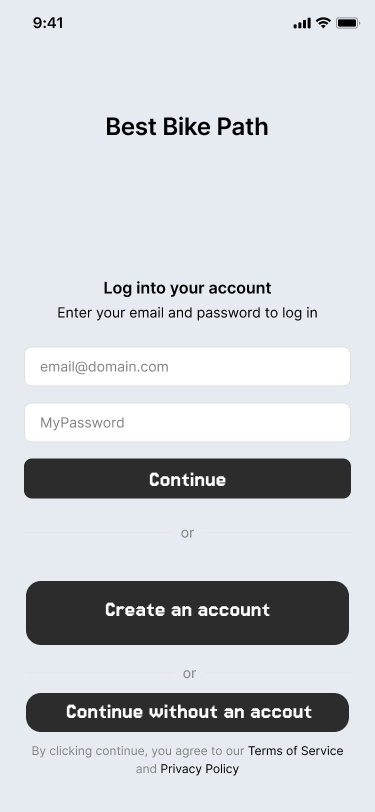
\includegraphics[width=0.4\linewidth]{RASD/Version1.0/images/Interfaces/Sign_In.png}
        \caption{Log in Interface} 
        \label{fig:log_in_interface}
    \end{center}
\end{figure}

Figure 3.1 represents the initial interface that any user encounters upon opening the application. From this screen, the user may choose to log in, sign up, or continue without creating an account, accessing a limited set of functionalities. 

\begin{figure}[H]
    \begin{center}
        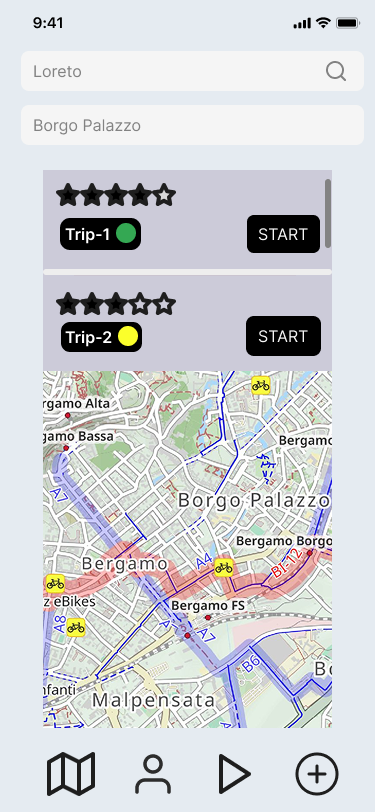
\includegraphics[width=0.4\linewidth]{RASD/Version1.0/images/Interfaces/Map_1.png}
        \caption{Map Interface} 
        \label{fig:Map_interface}
    \end{center}
\end{figure}

Figure 3.2 shows the map interface, which is displayed immediately after signing in or by selecting the map icon in the bottom navigation bar. At the top of the screen, a search bar allows the user to specify an origin and a destination in order to look for suitable cycling paths. Just below it, the suggested paths are presented, where the stars indicate the overall score of each path and the colored circle on the left represents the quality of the road. The map provides an overview of the available routes and serves as the central entry point for consulting path information and exploring the surrounding area.

\begin{figure}[H]
    \begin{center}
        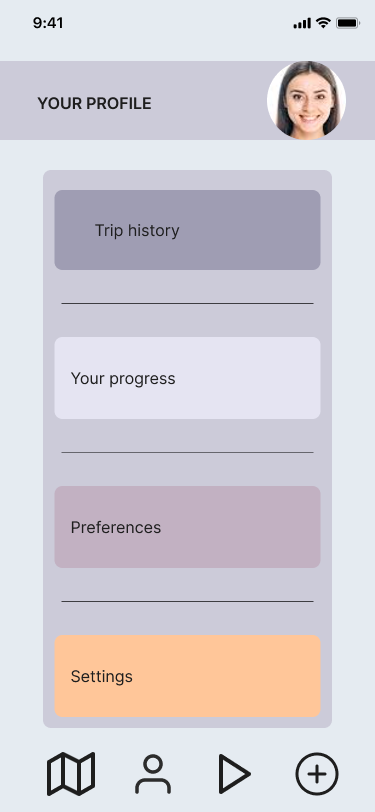
\includegraphics[width=0.4\linewidth]{RASD/Version1.0/images/Interfaces/Profile.png}
        \caption{Profile interface} 
        \label{fig:profile_interface}
    \end{center}
\end{figure}

Figure 3.3 illustrates the profile interface, which can be accessed by selecting the human-shaped icon in the bottom navigation bar. The \textit{Trip History} section displays all the user's completed trips and allows them to publish any unpublished paths as well as view detailed statistics for each ride. The \textit{Your Progress} section summarizes the user's overall activity, including metrics such as the total number of completed trips and the cumulative distance traveled. In the \textit{Preferences} section, the user can configure their preferred path qualities, enabling the system to provide personalized route suggestions. Finally, the \textit{Settings} section allows the user to modify their account information, such as changing their profile picture or deleting their account.

\begin{figure}[H]
    \begin{center}
        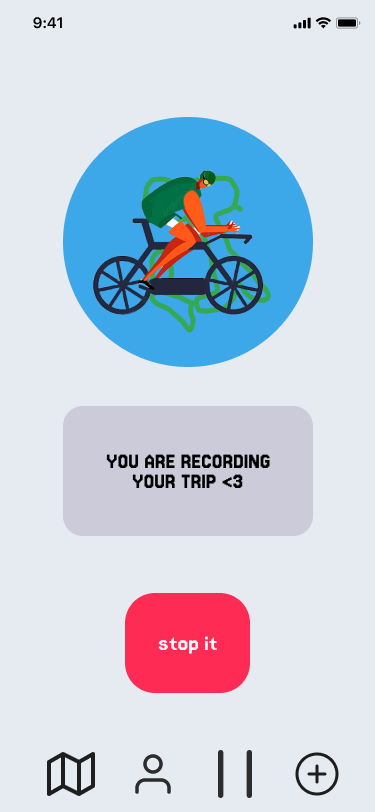
\includegraphics[width=0.4\linewidth]{RASD/Version1.0/images/Interfaces/Automatic 1.png}
        \caption{Automatic trip interface} 
        \label{fig:automatic_interface}
    \end{center}
\end{figure}

Figure 3.4 shows the interface displayed after pressing the start button in the bottom navigation bar, which initiates the automatic trip detection mode. During this mode, the system records the user's movement and collects sensor data to reconstruct the traveled path. The trip can be terminated at any time either by pressing the \textit{Stop} button on the screen or by selecting the same bottom navigation button, which now functions as a stop control. While the trip is being recorded, the user may continue to navigate and use the application freely without interrupting the ongoing detection process.

\begin{figure}[H]
    \begin{center}
        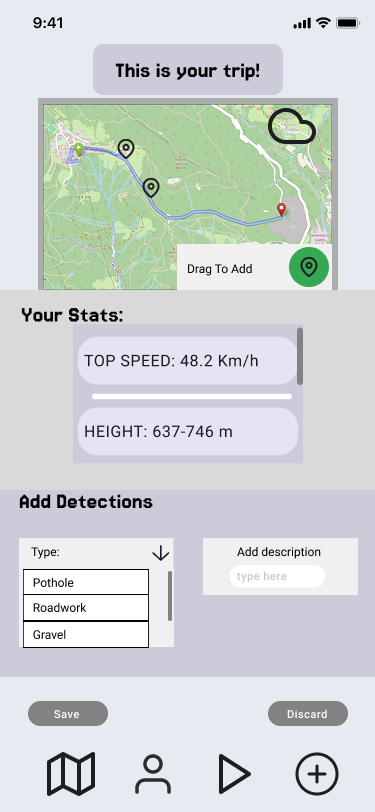
\includegraphics[width=0.4\linewidth]{RASD/Version1.0/images/Interfaces/Automatic 2.png}
        \caption{Detection confirmation interface} 
        \label{fig:automatic_detection}
    \end{center}
\end{figure}

Figure 3.5 shows the interface displayed after stopping the automatic trip detection illustrated in Figure 3.4. In this screen, the user can review the statistics of the completed trip and examine the automatically detected events. The lower section allows the user to add new detections or modify the ones suggested by the system. To precisely indicate where a detection occurred, the user can drag the pin on the map, positioning it on the exact road segment where the event took place.

\begin{figure}[H]
    \begin{center}
        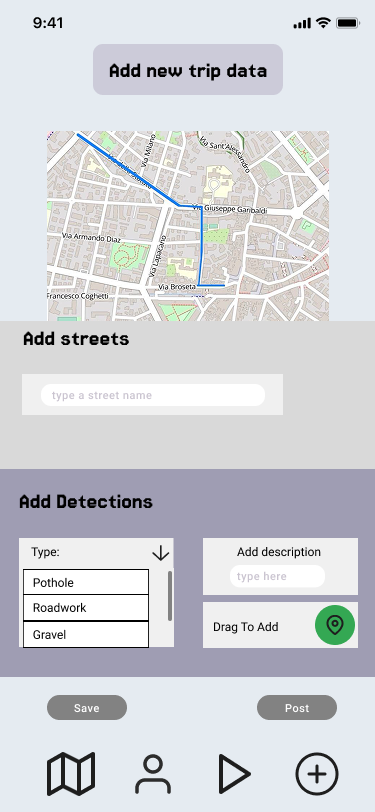
\includegraphics[width=0.4\linewidth]{RASD/Version1.0/images/Interfaces/Manual 1.png}
        \caption{Manual trip interface} 
        \label{fig:manual_interface}
    \end{center}
\end{figure}

Figure 3.6 can be accessed by pressing the ``+'' icon in the bottom navigation bar, allowing the user to create a trip manually. In this interface, the user may build a route by entering the names of the streets or by selecting their beginning and end points by clicking directly on the map and choosing an existing path between the two points. The blue lines represent the selected street segments. Once the route has been created, the user may continue forward to add the detections by pressing the \textit{Confirm path} button. In the following screen after having added the desired detections the user has the ability to either save the trip in his history or to directly post it as a contribution without saving it in his account.


\subsection{Hardware Interfaces}

The system shall ensure full compatibility with the hardware components involved in the interaction between users' devices and the platform. The following requirements apply:

\subsubsection*{User Devices}
\begin{itemize}
    \item The platform shall support access from a wide range of commonly used device such as tablets and smartphones. %mi sembra follia mettere anche tablet ma mi sembrava restrittivo dire solo smartphones 
    
    \item The platform shall be fully usable across different screen sizes and resolutions, ensuring responsiveness and readability regardless of device type.

    \item User devices shall include sufficient storage and processing capabilities to run the mobile application, including support for caching data and executing client-side scripts.

    \item For devices using automatic trip detection or sensor-based functionalities, the system shall interface with hardware components such as \textbf{GPS receivers}, \textbf{accelerometers}, and \textbf{gyroscopes}. These components must be accessible to the application for acquiring motion data, trip-related information, and geolocation.% non so se ha più senso in software o in hardware ma non metterei in entrambi
    
\end{itemize}


\subsection{Software Interfaces}

The system is designed as a mobile application, capable of performing all its core functionalities without relying on essential third-party software. Nevertheless, the system shall comply with the following software interface requirements:

\begin{itemize}
    \item The system shall function correctly across the most widely adopted operating systems, such as \textbf{Android}, and \textbf{iOS}.
    
    \item The system shall interface with geolocation and mapping services to retrieve, compute, and display cycling routes. These services include GPS modules, map-rendering libraries, and geocoding/route-search components.
    
    \item The system shall interface with external meteorological information providers to retrieve weather conditions relevant to trips and route safety evaluations and with external map service providers to retrieve geographical data.
    
    \item The system shall interact with mobile device sensors, including accelerometer and gyroscope, to collect motion-related data supporting the automatic detection of obstacles and road conditions.
    
    \item No additional software installations or configurations shall be required on the user's device, aside from using the official mobile application.
\end{itemize}

\subsection{Communication Interfaces}

The system shall support reliable and secure communication mechanisms enabling interaction between client devices, backend services, and external data providers. The following requirements apply:

\begin{itemize}
    \item The system shall operate over standard Internet connections, such as \textbf{Wi-Fi}, and \textbf{mobile data}.
    
    \item All communication between the client and the server shall be secured through \textbf{encrypted protocols} (e.g., TLS/SSL) to protect sensitive information such as user credentials, personal data, recorded trips, and sensor-based contributions.
    
    \item The system shall utilize widely adopted \textbf{web communication protocols}, primarily \textbf{HTTPS}, to ensure secure and reliable data transmission between user devices and the backend.
    
    \item The system shall support communication with external services, including meteorological data providers and geolocation/map services, through standard \textbf{HTTP/HTTPS-based APIs}.
    
    \item No additional software installations or communication packages shall be required on the user’s device to enable proper communication with the platform.
    
    \item The system shall minimize communication latency by adhering to industry-standard response times ensuring a smooth and responsive user experience.
\end{itemize}


\subsubsection*{Hosting Infrastructure}
\begin{itemize}
    \item The system shall be deployed on a hosting infrastructure capable of supporting simultaneous access by multiple users with minimal latency.
    
    \item The hosting environment shall provide sufficient computational resources for processing real-time map data, aggregating user contributions, and executing background operations.

    \item The infrastructure shall include adequate storage capabilities to manage user profiles, trips, sensor data, and historical records of contributions.

    \item The hosting environment shall be scalable, allowing the system to accommodate increasing traffic, data volume, and computational demands over time while preserving service availability and performance.
\end{itemize}



\section{Functional Requirements}
\label{sec:functional_requirements}

\begin{figure}[H]
    \begin{center}
        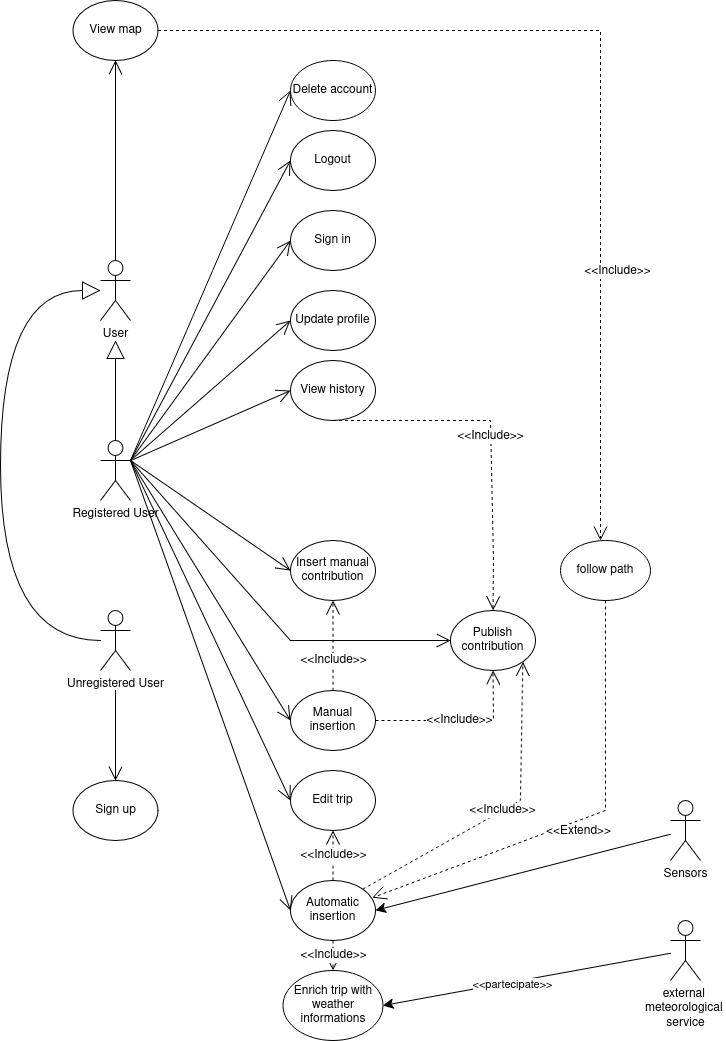
\includegraphics[width=0.9\linewidth]{RASD/Version1.0/images/use_case_diagram.png}
        \caption{Use Case Diagram} 
        \label{fig:use_case_diagram}
    \end{center}
\end{figure}

\newpage
\subsection{Use Cases and Activity Diagrams}
\label{subsec: use_cases}%

\newcounter{ucsteps}
\setcounter{ucsteps}{1}
\newcommand{\cucsteps}{\theucsteps\stepcounter{ucsteps}}
\newcommand{\resetucsteps}{\setcounter{ucsteps}{1}}

\newcounter{uc}
\setcounter{uc}{1}
\newcommand{\cuc}{\theuc\stepcounter{uc}\resetucsteps}

\subsubsection*{UC\cuc . Sign Up}
\begin{center}
    \begin{longtable}{|l|p{0.75\linewidth}|}
        \hline
        \textbf{Actor}            & User\\
        \hline
        \textbf{Entry Conditions} & The User is not logged into the platform and is on the homepage. \\
        \hline
        \textbf{Flow of Events}    
        & \cucsteps. On the homepage, the User clicks the ``Sign up'' button. \\
        & \cucsteps. The system displays the registration form. \\
        & \cucsteps. The User inserts the required registration details (e.g., email, password and password confirmation). \\
        & \cucsteps. The User confirms the provided information by clicking the ``Register'' button. \\
        & \cucsteps. The system checks the completeness and validity of the submitted data. \\
        & \cucsteps. If the data is valid, the system sends a confirmation email containing a verification link that expires after 24 hours. \\
        & \cucsteps. The User clicks the confirmation link in the email before it expires. \\
        & \cucsteps. The system allows the User to access the profile page and complete the profile by inserting the remaining personal details. \\
        \hline
        \textbf{Exit Conditions}   & The User account is created and verified, and the profile is completed so that the User can access the platform functionalities.\\       
        \hline
        \textbf{Exceptions}       & \begin{itemize}[leftmargin=*]
            \item Some mandatory fields are missing: the system notifies ``Missing mandatory fields'' and does not allow the User to proceed until all required fields are filled in.
            \item The password does not satisfy the platform's security requirements: the system notifies ``Invalid password'' and prompts the User to correct it.
            \item The email address is already linked to an existing account: the system notifies ``Email already linked'' and redirects the User to the login page.
            \item The confirmation link expires before being used: the system discards all data previously inserted by the User and invalidates the link.
        \end{itemize} \\
        \hline
    \end{longtable}
\end{center}


\begin{figure}[H]
    \begin{center}
         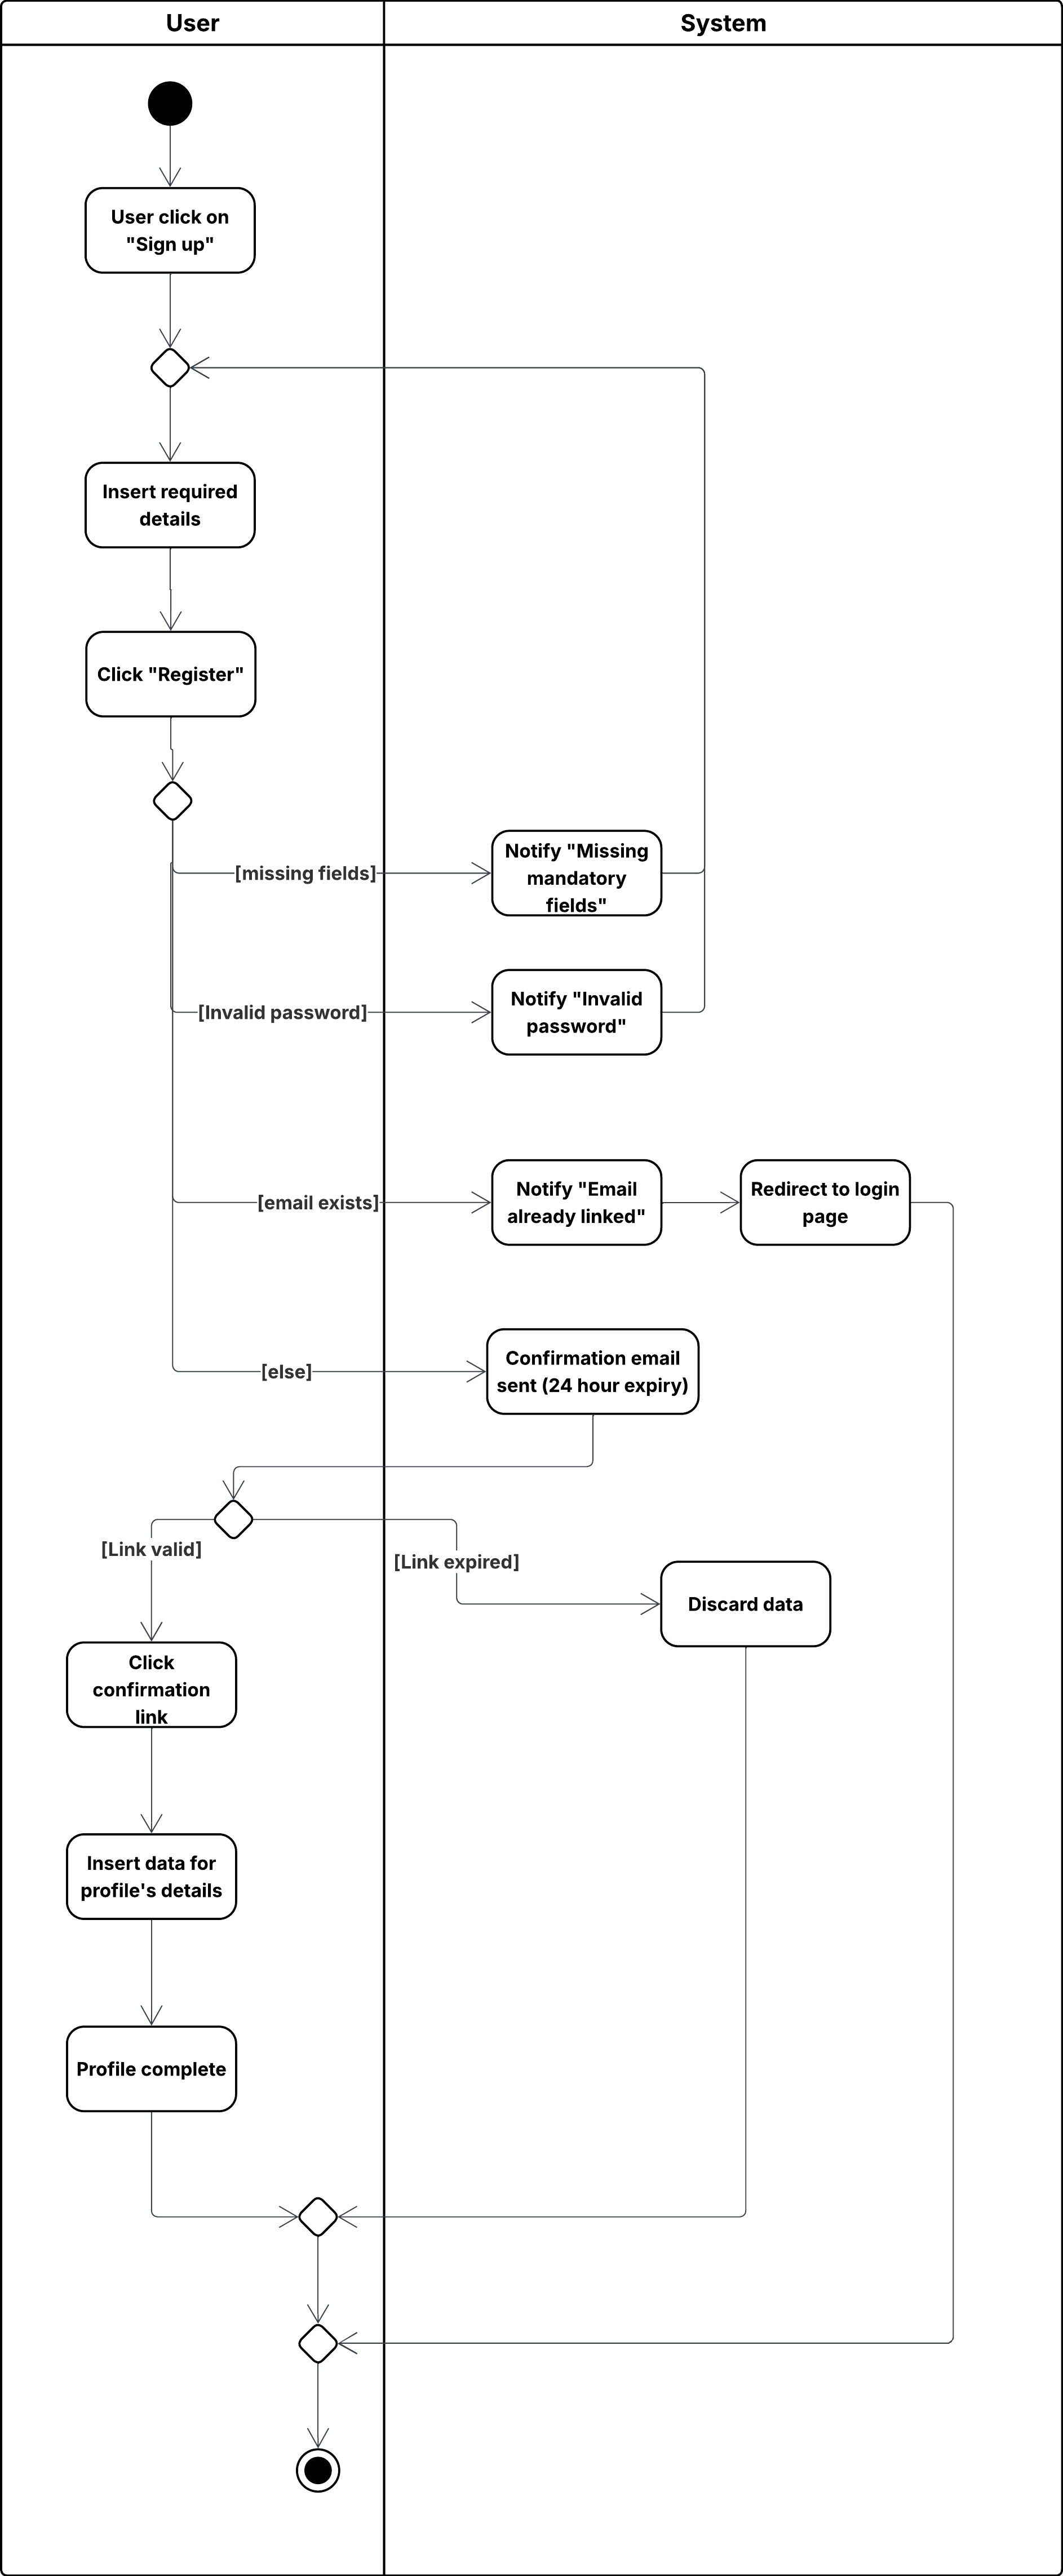
\includegraphics[width=0.5\linewidth]{RASD/Version1.0/images/activity diagram/UC1.png}
         \caption{Sign Up}
         \label{fig:signup_student_ad}
     \end{center}
\end{figure}

\newpage


\subsubsection*{UC\cuc . Sign In}
\begin{center}
    \begin{longtable}{|l|p{0.75\linewidth}|}
        \hline
        \textbf{Actor}            & User \\
        \hline
        \textbf{Entry Conditions} & The User is not logged into the platform and is on the homepage. \\
        \hline
        \textbf{Flow of Events}    
        & \cucsteps. On the homepage, the User clicks the ``Sign in'' button. \\
        & \cucsteps. The system displays the login form. \\
        & \cucsteps. The User enters their credentials (email and password). \\
        & \cucsteps. The User clicks the ``Login'' button to submit the credentials. \\
        & \cucsteps. The system validates the provided credentials. \\
        & \cucsteps. If the credentials are valid and the account is verified, the system checks whether the User's profile is complete. \\
        & \cucsteps. If the profile is complete, the system redirects the User to the Home page. \\
        & \cucsteps. If the profile is not complete, the system redirects the User to the ``Update profile'' page. \\
        \hline
        \textbf{Exit Conditions}   & The User is successfully authenticated and is redirected either to the Home page or to the profile completion page.\\
        \hline
        \textbf{Exceptions}       & {%
            \begin{itemize}[leftmargin=*]
                \item The entered credentials are not valid: the system notifies ``Entered credentials are not valid'' and does not log the User in.
                \item The account associated with the provided email is not verified: the system notifies ``Account not verified'' and does not log the User in.
            \end{itemize}
        } \\
        \hline
    \end{longtable}
\end{center}



\begin{figure}[H]
    \begin{center}
         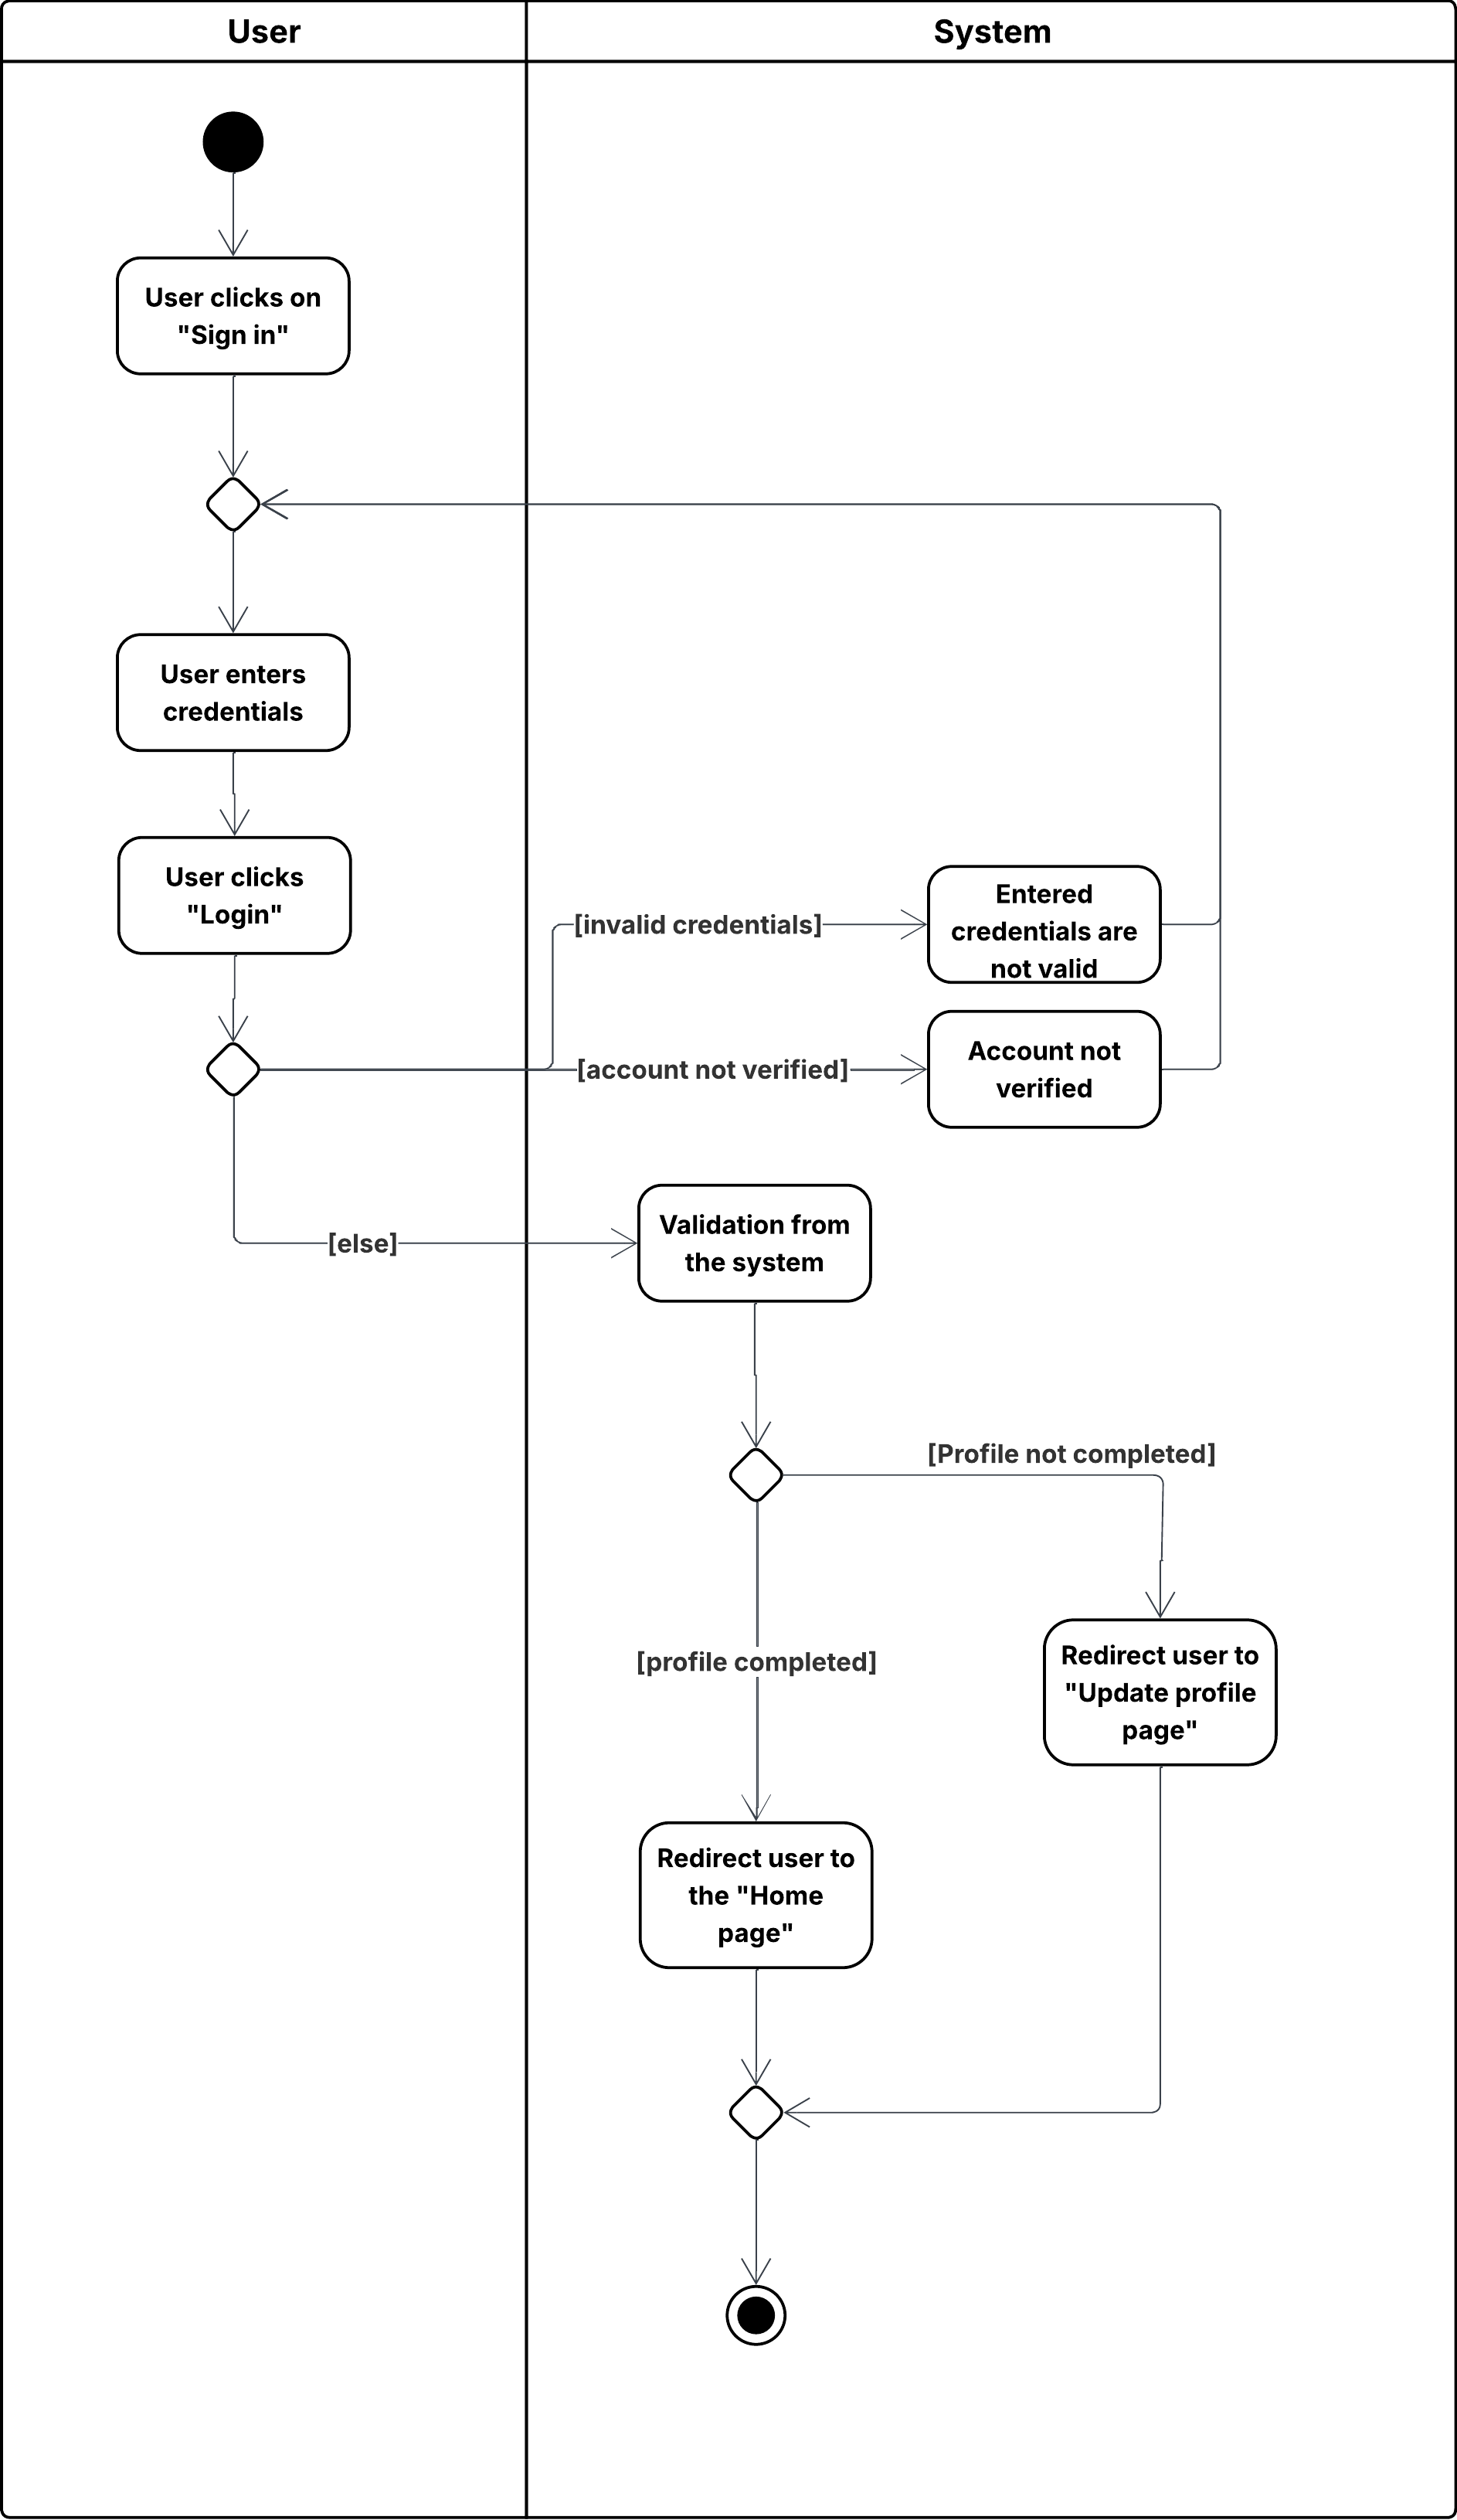
\includegraphics[width=0.5\linewidth]{RASD/Version1.0/images/activity diagram/UC2.png}
         \caption{Sign In}
         \label{fig:signin}
     \end{center}
\end{figure}

\newpage


\subsubsection*{UC\cuc . Delete Account}
\begin{center}
    \begin{longtable}{|l|p{0.75\linewidth}|}
        \hline
        \textbf{Actor}            & Registered User \\
        \hline
        \textbf{Entry Conditions} & The Registered User is logged into the platform and is on the account settings page. \\
        \hline
        \textbf{Flow of Events}    
        & \cucsteps. The User opens the account settings section. \\
        & \cucsteps. The User selects the ``Delete account'' option. \\
        & \cucsteps. The system shows a warning explaining the consequences of account deletion and asks the User whether they want to continue. \\
        & \cucsteps. The User confirms the intention to proceed with account deletion. \\
        & \cucsteps. The system requests re-authentication by asking the User to enter their credentials. \\
        & \cucsteps. The User inserts their credentials and submits them. \\
        & \cucsteps. The system validates the provided credentials. \\
        & \cucsteps. If the credentials are valid, the system removes the User profile and related personal information. \\
        & \cucsteps. The system deletes the trips stored for the User. \\
        & \cucsteps. The system deletes the User's preferences and local settings. \\
        & \cucsteps. The system invalidates any active sessions and authentication tokens associated with the User. \\
        & \cucsteps. The system notifies the User that the account has been successfully deleted. \\
        \hline
        \textbf{Exit Conditions}   & The User account and all associated data are deleted, and the User is no longer able to access the platform with the previous credentials.\\
        \hline
        \textbf{Exceptions}       & {%
            \begin{itemize}[leftmargin=*]
                \item The User cancels the deletion after viewing the warning: the system returns the User to the account settings page without performing any deletion.
                \item The re-authentication credentials are not valid: the system notifies the User that the credentials are invalid and returns to the account settings page without deleting the account.
            \end{itemize}
        } \\
        \hline
    \end{longtable}
\end{center}


\begin{figure}[H]
    \begin{center}
         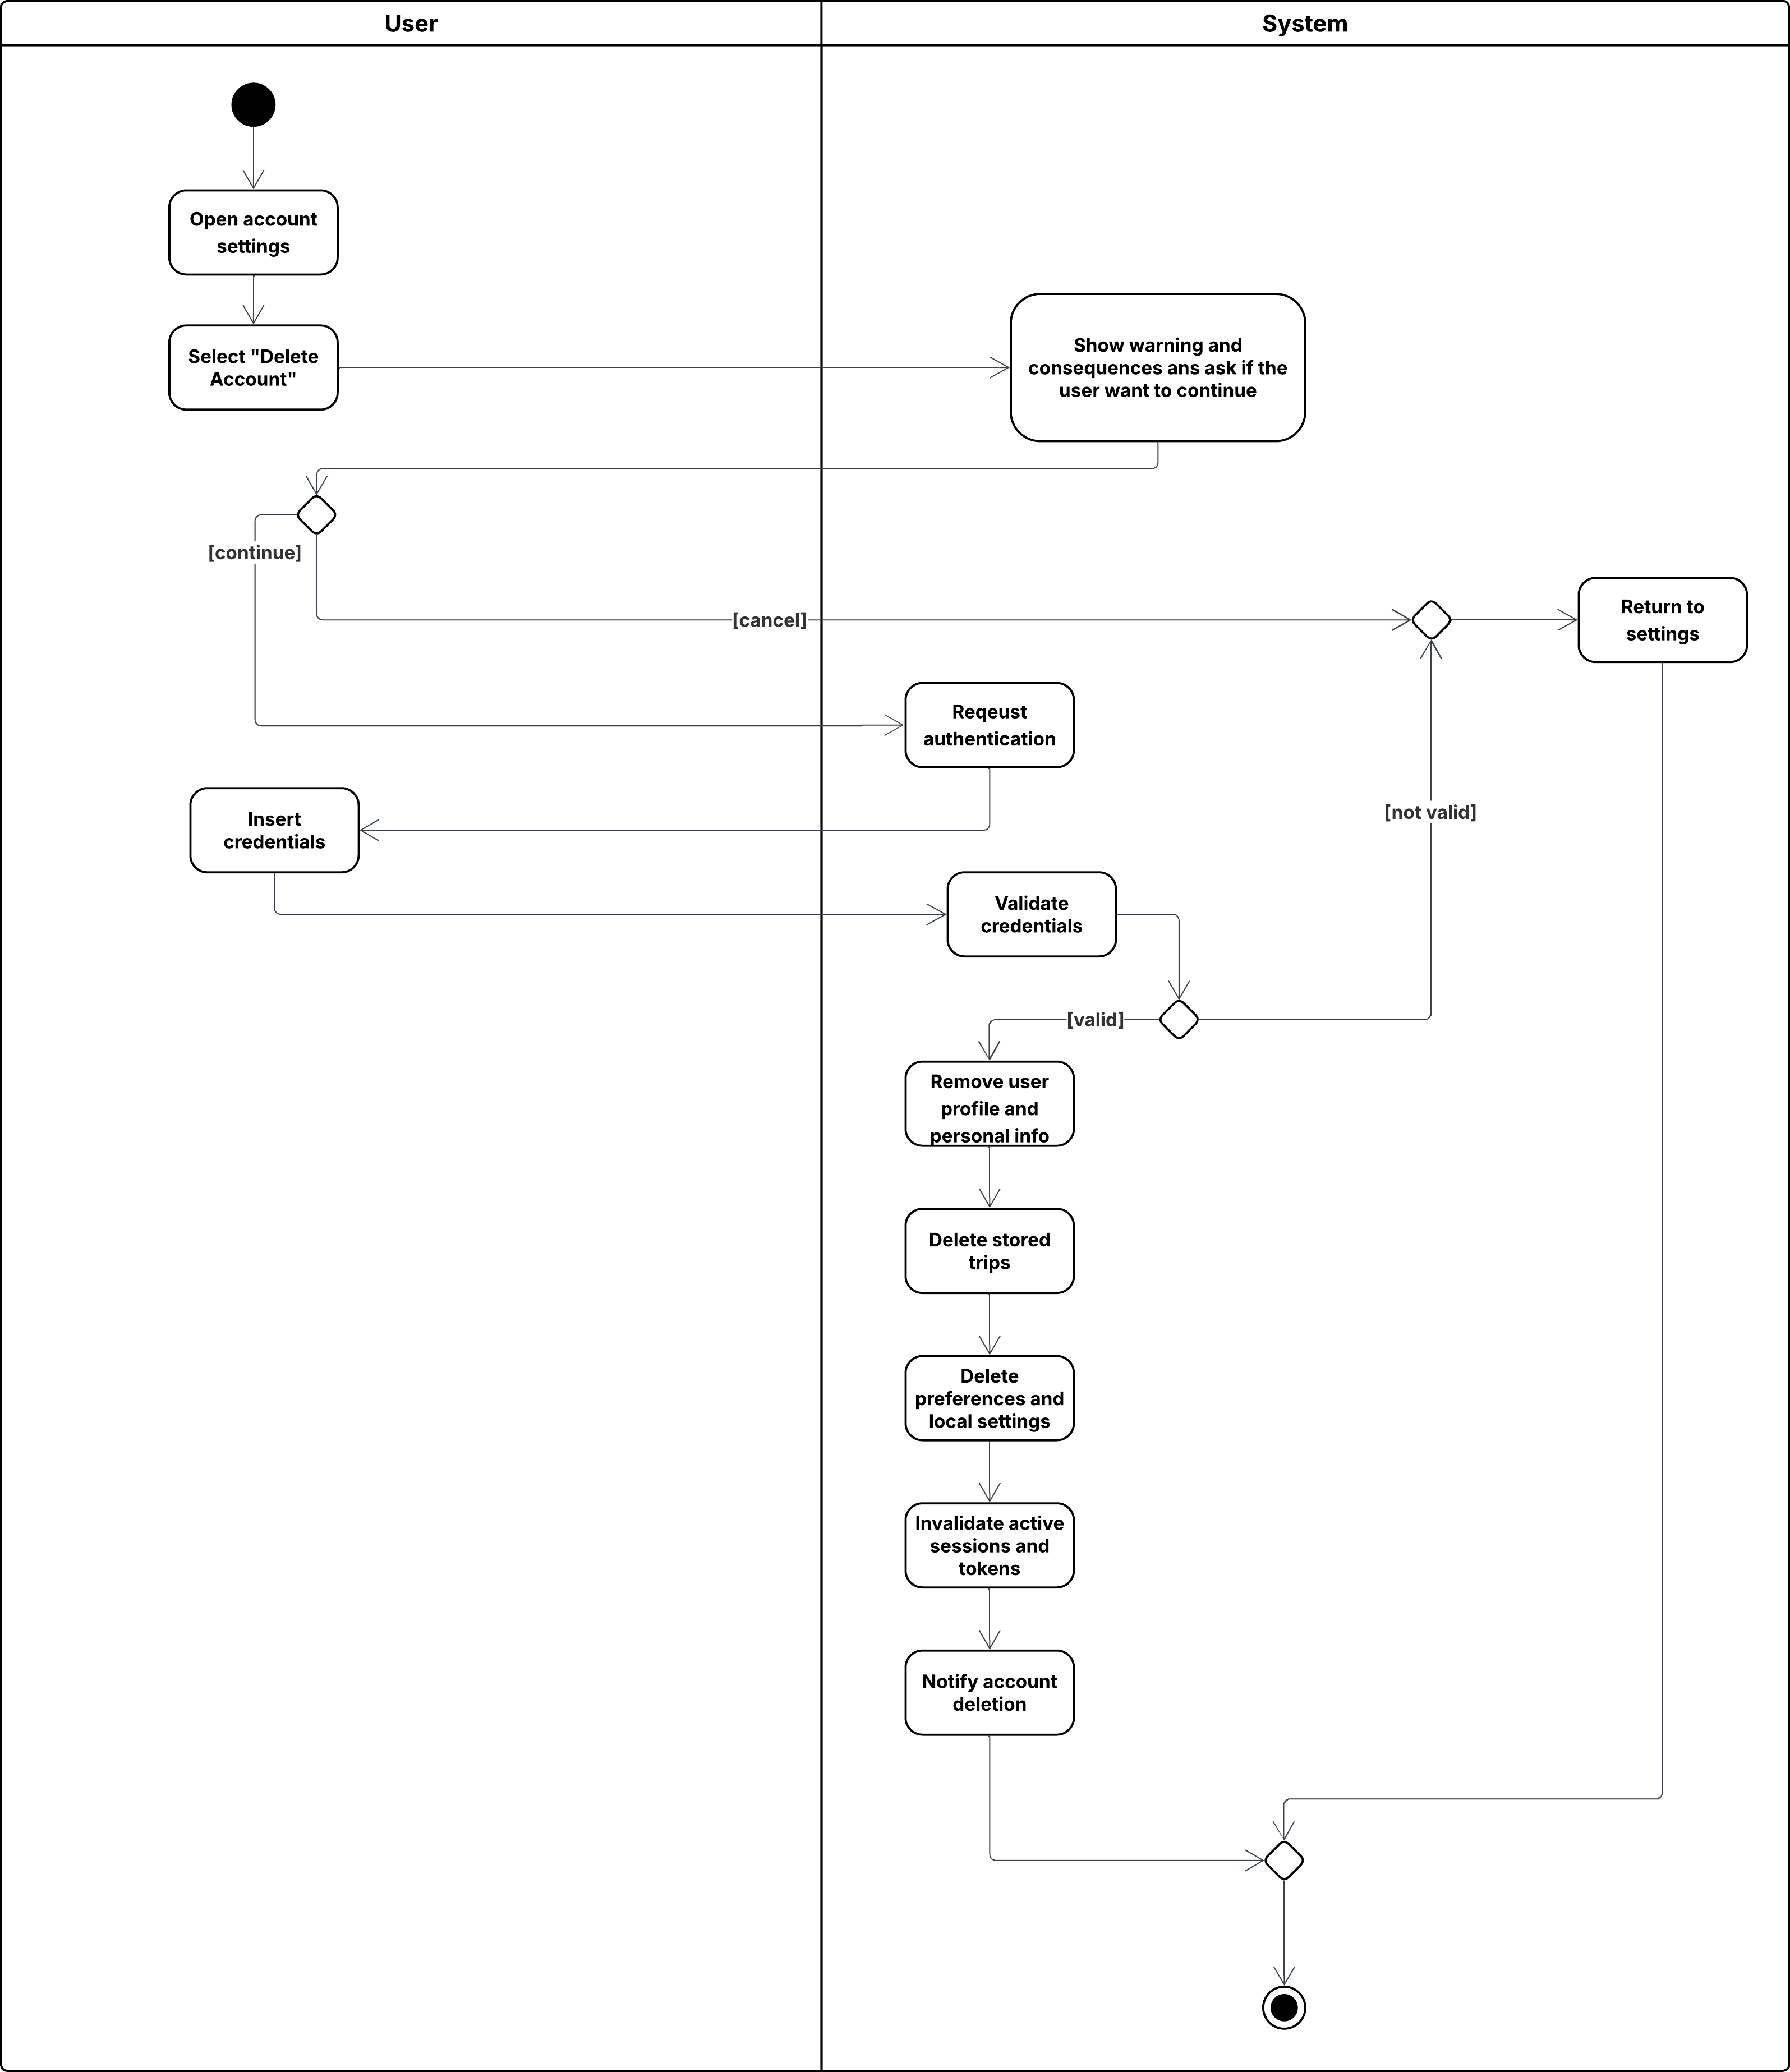
\includegraphics[width=0.9\linewidth]{RASD/Version1.0/images/activity diagram/UC3.png}
         \caption{Delete Account}
         \label{fig:delete_account}
     \end{center}
\end{figure}

\newpage


\subsubsection*{UC\cuc . Logout}
\begin{center}
    \begin{longtable}{|l|p{0.75\linewidth}|}
        \hline
        \textbf{Actor}            & User \\
        \hline
        \textbf{Entry Conditions} & The User is logged into the platform. \\
        \hline
        \textbf{Flow of Events}    
        & \cucsteps. The User clicks on the ``Logout'' button. \\
        & \cucsteps. The system receives the logout request. \\
        & \cucsteps. The system terminates the User's session and invalidates any active authentication token. \\
        & \cucsteps. The system redirects the User to the Home screen. \\
        \hline
        \textbf{Exit Conditions}   & The User's session is terminated, and the User is no longer authenticated on the platform.\\
        \hline
        \textbf{Exceptions}       & {%
            \begin{itemize}[leftmargin=*]
                \item None.
            \end{itemize}
        } \\
        \hline
    \end{longtable}
\end{center}




\begin{figure}[H]
    \begin{center}
         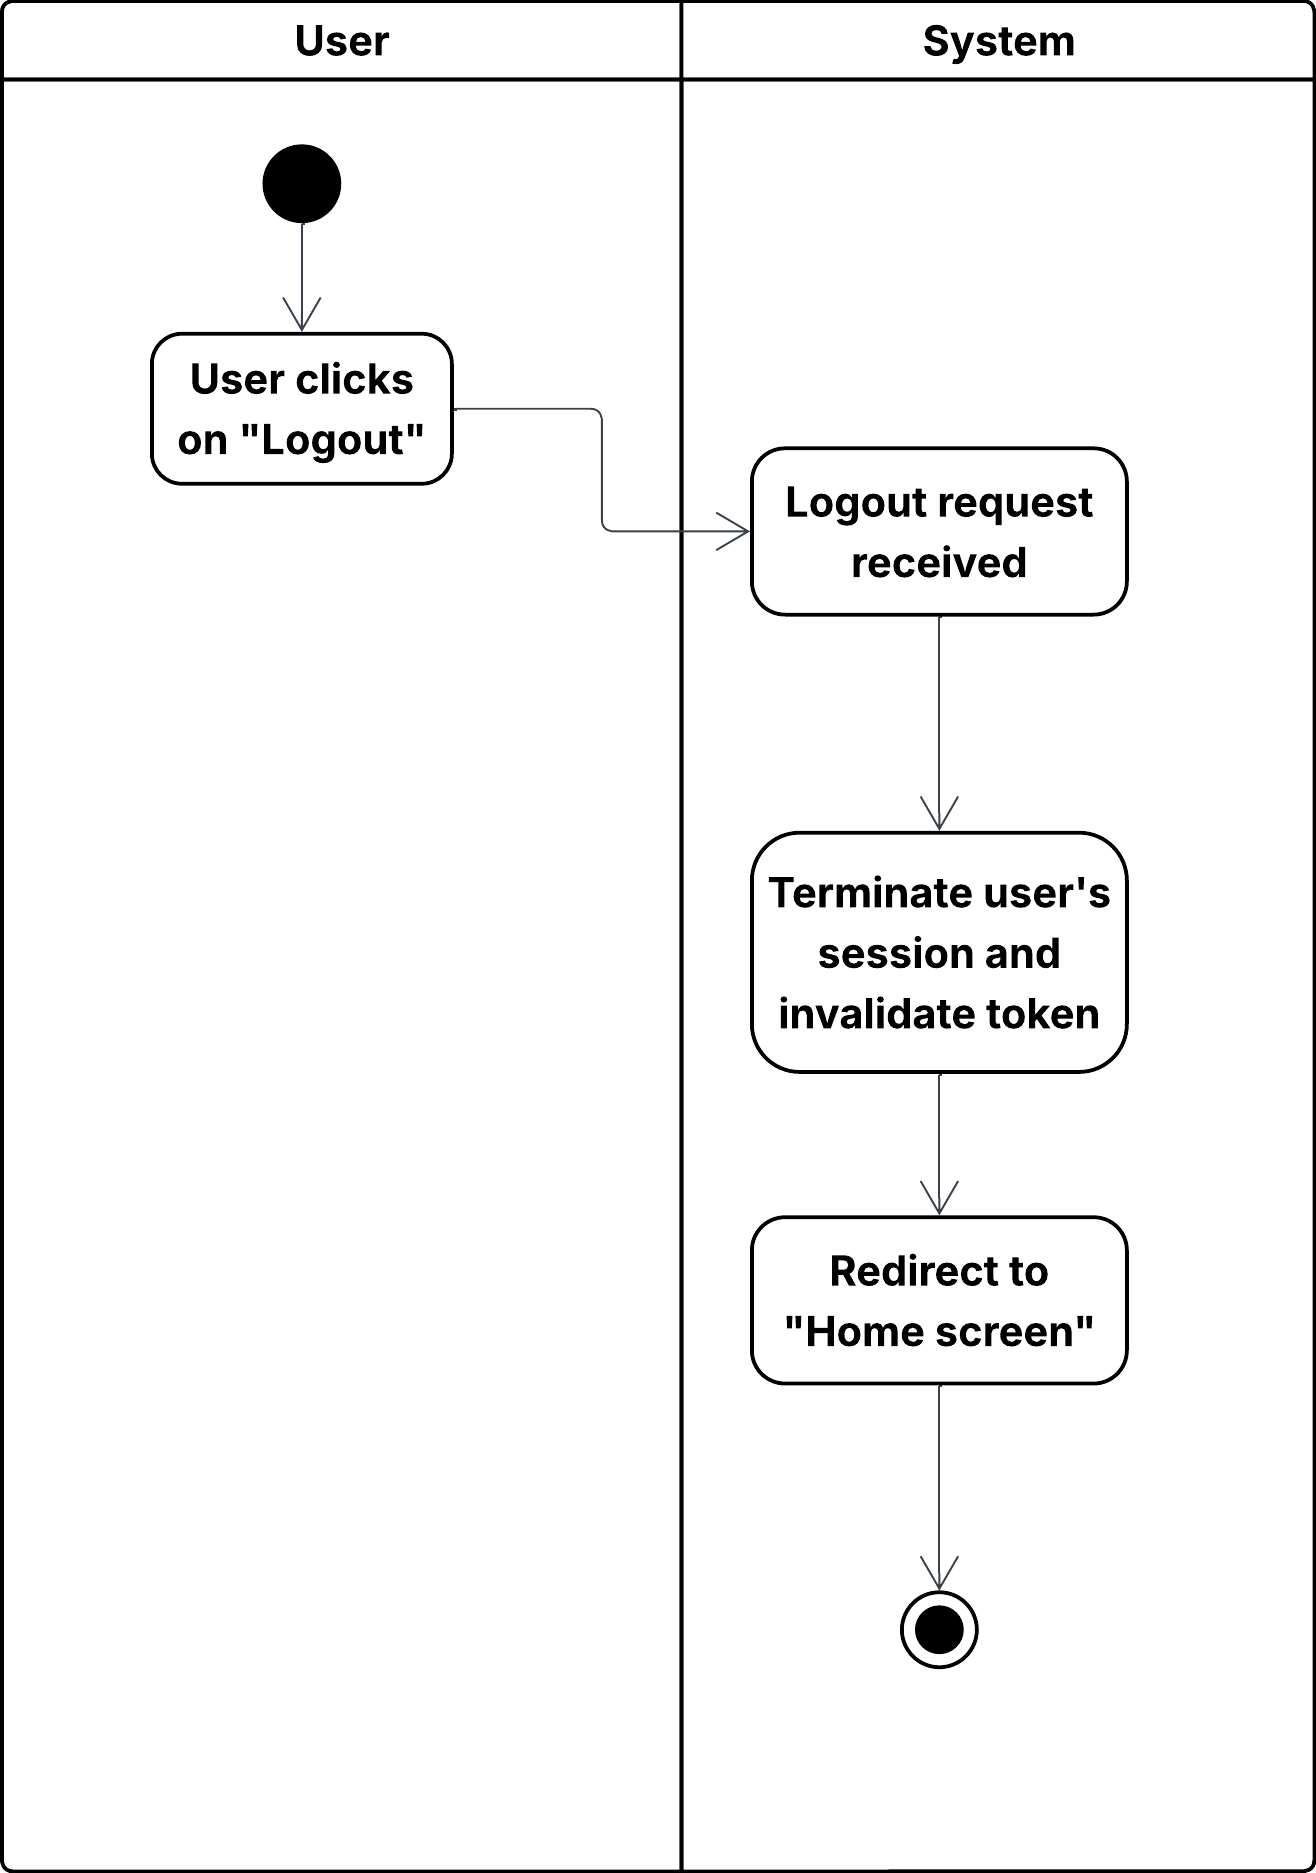
\includegraphics[width=0.9\linewidth]{RASD/Version1.0/images/activity diagram/UC4.png}
         \caption{Logout}
         \label{fig:Logout}
     \end{center}
\end{figure}

\newpage

\subsubsection*{UC\cuc . Edit Profile}
\begin{center}
    \begin{longtable}{|l|p{0.75\linewidth}|}
        \hline
        \textbf{Actor}            & Registered User \\
        \hline
        \textbf{Entry Conditions} & The Registered User is logged into the platform. \\
        \hline
        \textbf{Flow of Events}    
        & \cucsteps. The User clicks on the ``Profile'' section. \\
        & \cucsteps. The User clicks on the ``Edit profile'' option inside the settings. \\
        & \cucsteps. The system displays the editable profile form, including personal data and preference fields. \\
        & \cucsteps. The User updates the desired information, such as personal details and visualization preferences (e.g., preferred path filters based on past trips). \\
        & \cucsteps. The User clicks the ``Apply'' button to confirm the changes. \\
        & \cucsteps. The system validates the submitted changes. \\
        & \cucsteps. If the changes are valid, the system stores them and notifies the User of the successful update. \\
        \hline
        \textbf{Exit Conditions}   & The User's profile and preferences are updated and consistently stored in the system.\\
        \hline
        \textbf{Exceptions}       & {%
            \begin{itemize}[leftmargin=*]
                \item Some updated fields are not valid (e.g., invalid email format or unsupported preference values): the system notifies the User that the changes are not valid and does not apply them.
            \end{itemize}
        } \\
        \hline
    \end{longtable}
\end{center}


\begin{figure}[H]
    \begin{center}
         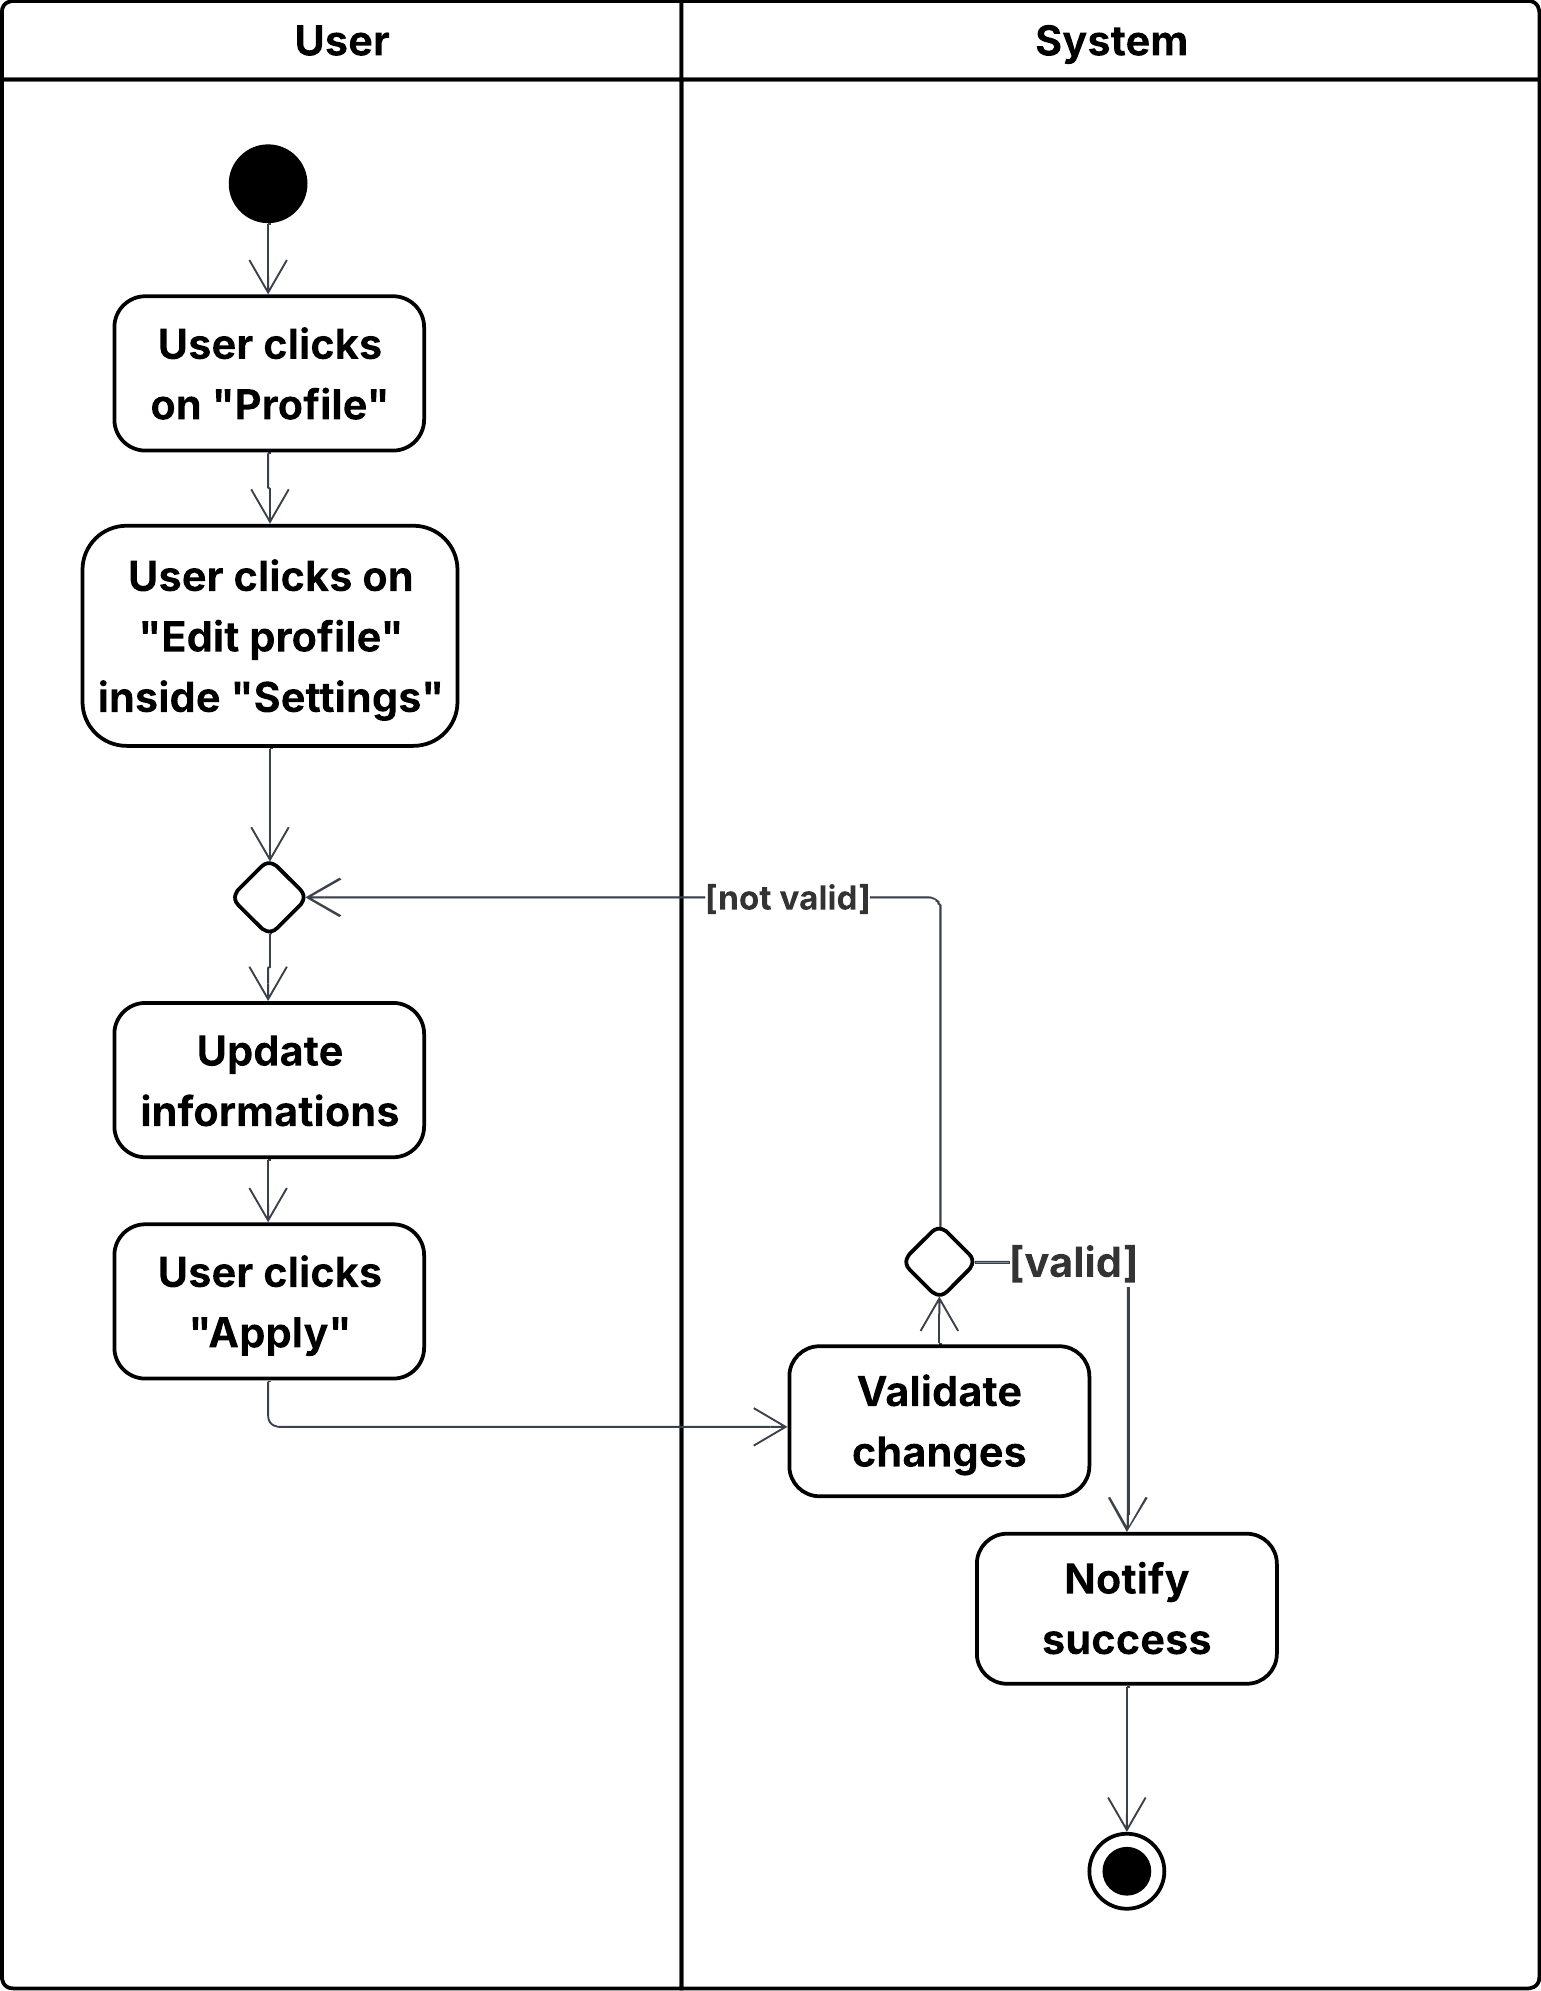
\includegraphics[width=0.9\linewidth]{RASD/Version1.0/images/activity diagram/UC5.png}
         \caption{Edit Profile}
         \label{fig:edit_profile}
     \end{center}
\end{figure}

\newpage

\subsubsection*{UC\cuc . View Trip History}
\begin{center}
    \begin{longtable}{|l|p{0.75\linewidth}|}
        \hline
        \textbf{Actor}            & Registered User \\
        \hline
        \textbf{Entry Conditions} & The Registered User is logged into the platform. \\
        \hline
        \textbf{Flow of Events}    
        & \cucsteps. The User clicks on the ``My trips'' section. \\
        & \cucsteps. The system retrieves the trips associated with the User and shows the list of available trips. \\
        & \cucsteps. The User selects one trip from the list. \\
        & \cucsteps. The system shows the selected trip together with its stored data and associated contributions. \\
        & \cucsteps. The User chooses an action for the selected trip (e.g., to publish its contributions or to simply inspect the data). \\
        & \cucsteps. If the User decides to publish the contributions of the trip, the system starts the \hyperref[sec:publish_contribution]{\uline{UC.~Publishing Contribution}} use case for the first contribution associated with that trip. \\
        & \cucsteps. The system iteratively processes the contributions linked to the trip, publishing them one at a time so that merge and update policies on paths can be correctly applied for each contribution. \\
        & \cucsteps. When there are no more contributions to process, the system returns control to the trip view. \\
        & \cucsteps. For readability, the activity diagram omits the fact that the User can navigate back to previous pages (trip list or other sections of the app) at any point in the interaction. \\
        \hline
        \textbf{Exit Conditions}   & The User has viewed the selected trip and, if desired, has published the contributions associated with that trip.\\
        \hline
        \textbf{Exceptions}       & {%
            \begin{itemize}[leftmargin=*]
                \item The User has no stored trips: the system shows an empty list and may display an informative message.
                \item The selected trip has no associated contributions: the system shows the trip data but does not start the publishing process.
            \end{itemize}
        } \\
        \hline
    \end{longtable}
\end{center}


\begin{figure}[H]
    \begin{center}
         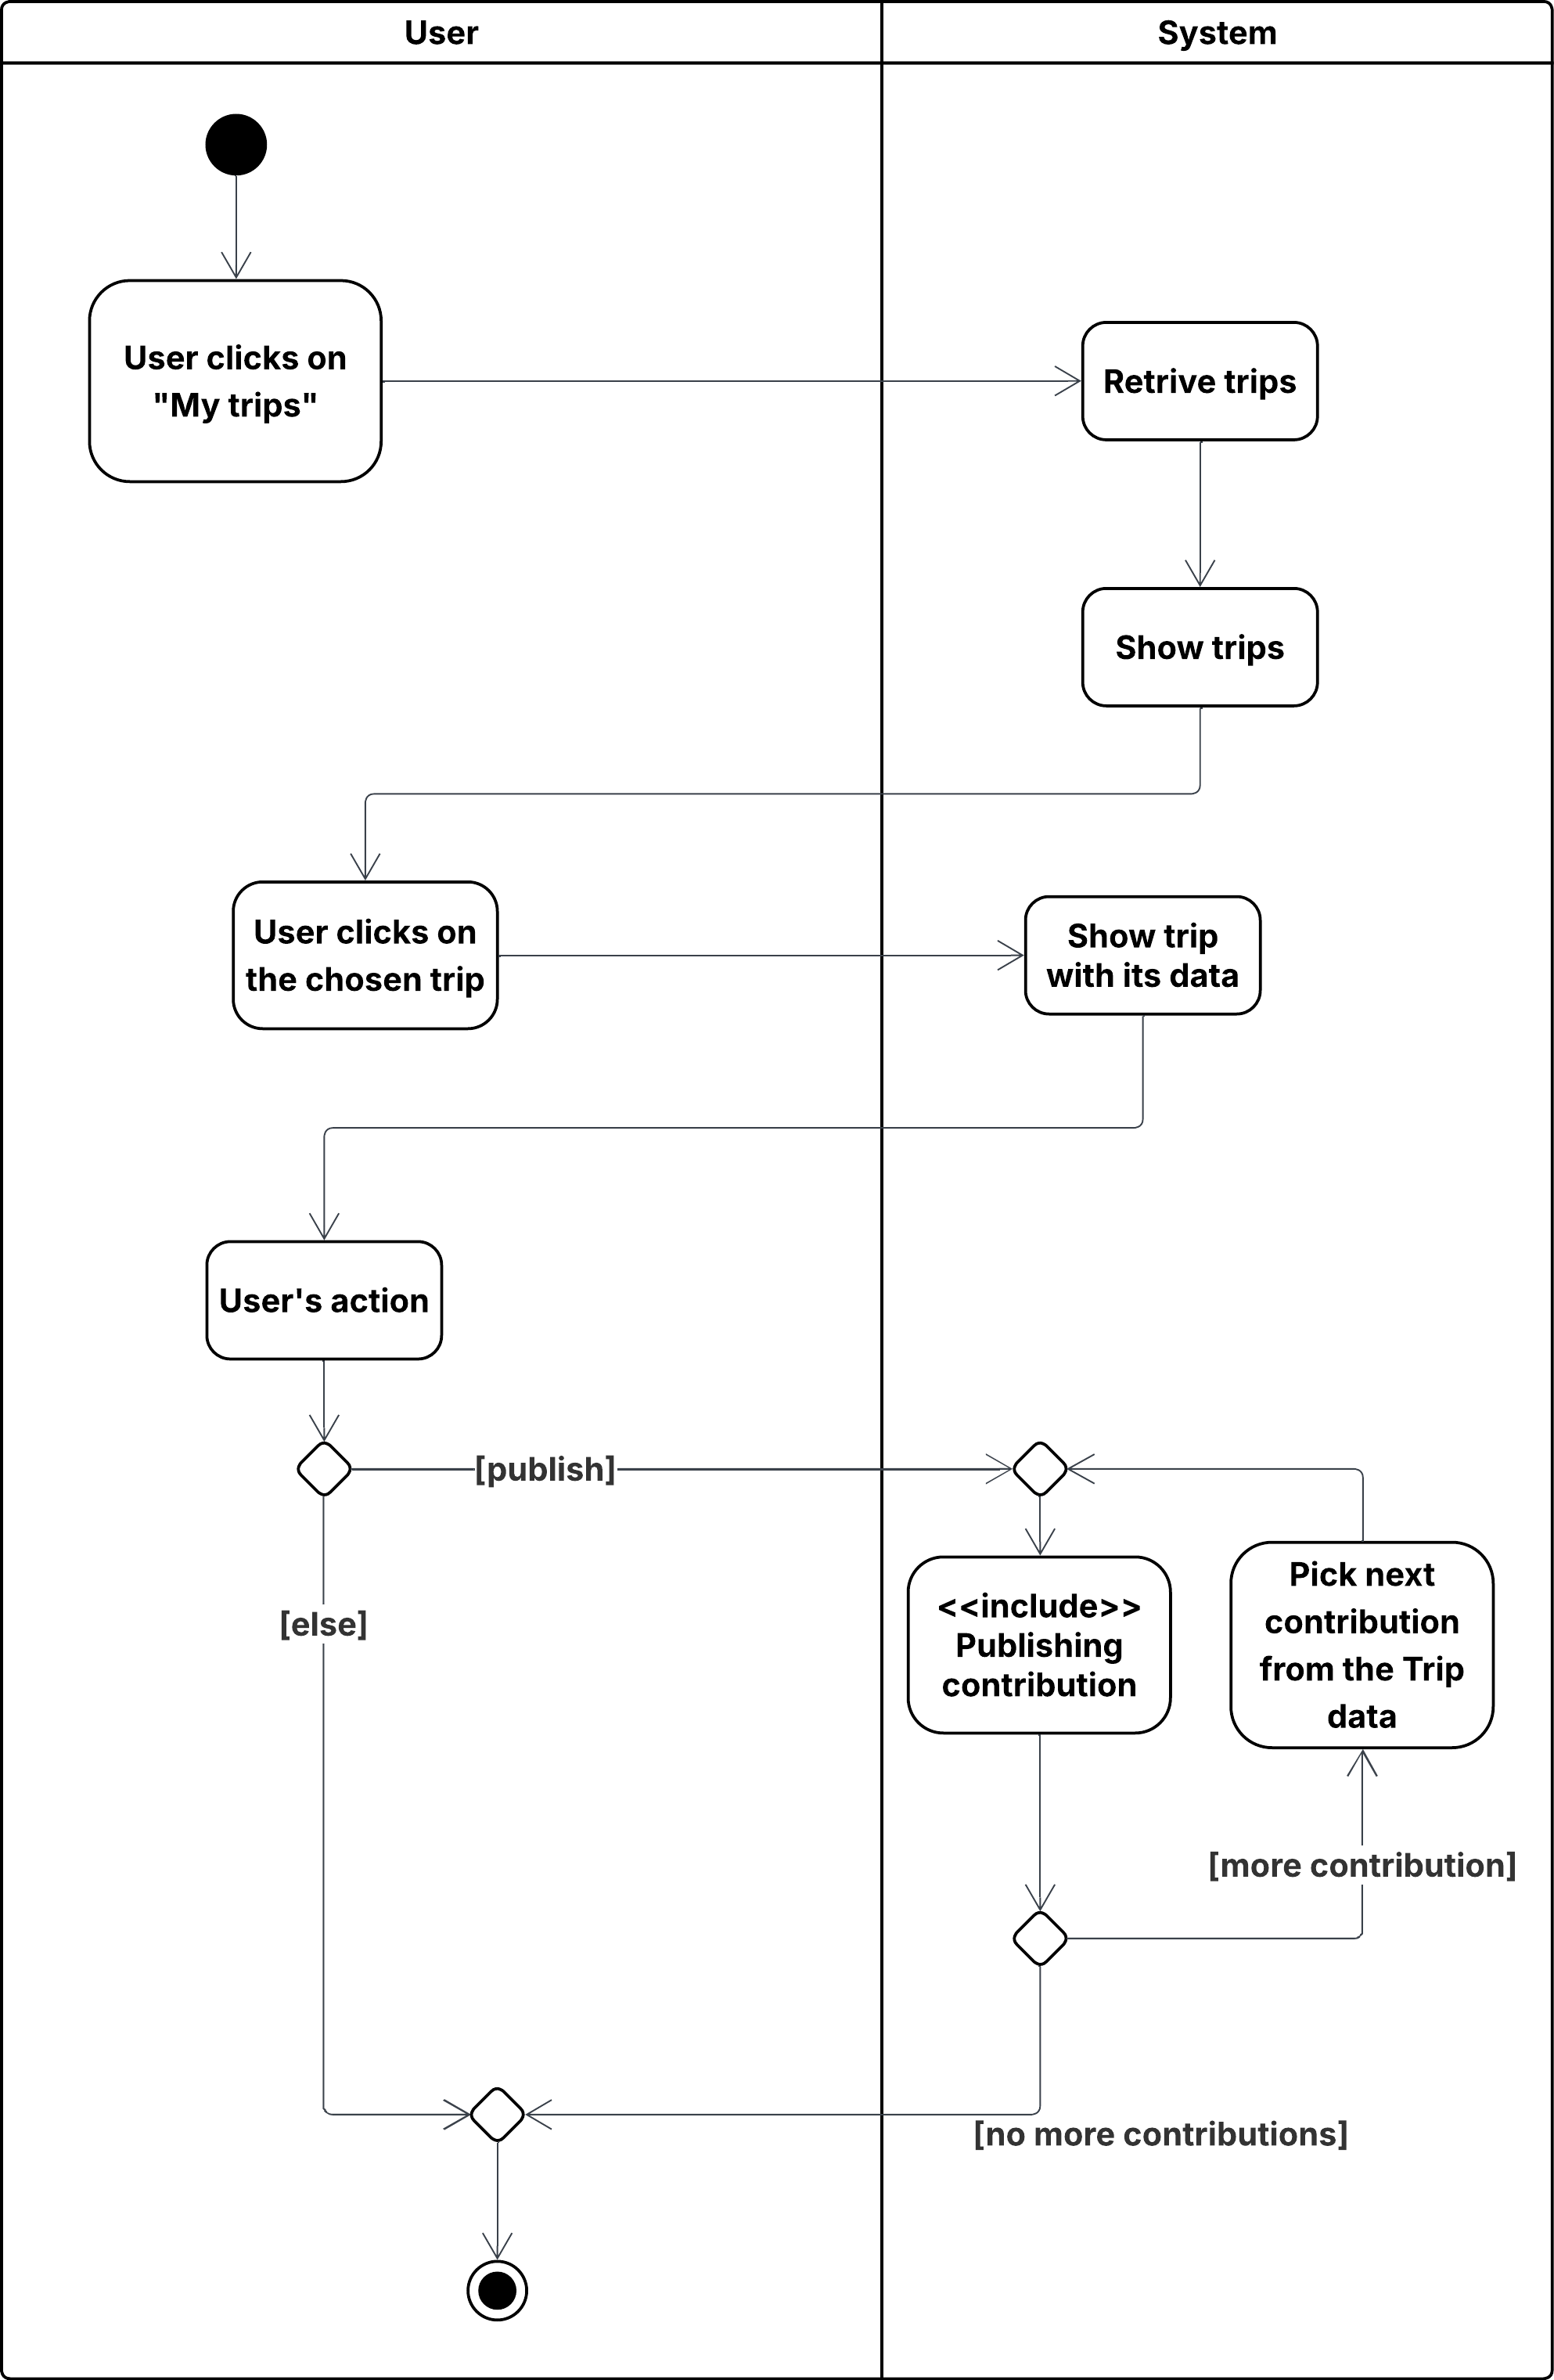
\includegraphics[width=0.9\linewidth]{RASD/Version1.0/images/activity diagram/UC6.png}
         \caption{View Trip History}
         \label{fig:view_trip_history}
     \end{center}
\end{figure}

\newpage




\subsubsection*{UC\cuc . Publish Contribution}
\label{sec:uc_publish_contribution}
\begin{center}
    \begin{longtable}{|l|p{0.75\linewidth}|}
        \hline
        \textbf{Actor}            & System (invoked from other use cases, e.g. View Trip History) \\
        \hline
        \textbf{Entry Conditions} & A Contribution has been selected for publication (for example, from a Trip in the User's history). \\
        \hline
        \textbf{Flow of Events}    
        & \cucsteps. The system validates the selected Contribution, checking that its data is complete and consistent. \\
        & \cucsteps. If the Contribution is valid, the system retrieves from the database any existing Contribution(s) referring to the same street or path segment. \\
        & \cucsteps. The system applies the configured merging policy to combine the new Contribution with the existing information (e.g., updating or aggregating obstacle data on that path). \\
        & \cucsteps. The system updates the corresponding path information in the database according to the result of the merging policy. \\
        & \cucsteps. The system flags the User's Contribution as published. \\
        & \cucsteps. The system notifies the successful publication of the Contribution to the invoking use case. \\
        \hline
        \textbf{Exit Conditions}   & The Contribution is marked as published and the affected path information in the database has been updated according to the merging policy.\\
        \hline
        \textbf{Exceptions}       & {%
            \begin{itemize}[leftmargin=*]
                \item The Contribution is not valid (e.g., missing mandatory data or inconsistent location): the system notifies the failure and does not modify any existing path information.
                \item A database error occurs while retrieving or updating existing Contributions: the system notifies the failure and leaves the User's Contribution in a non-published state.
            \end{itemize}
        } \\
        \hline
    \end{longtable}
\end{center}

\paragraph{Important Note}
This use case describes the \emph{conceptual} behavior of the system from the perspective of the involved stakeholders.  
In particular, it does not reflect the actual implementation details of the publication process, which, as discussed in the Design Document, is realized through an asynchronous mechanism.  

The use case abstracts away such implementation aspects and focuses instead on what should logically occur and on what the registered user is expected to perceive in terms of system behavior and outcomes, regardless of the underlying execution model.


\begin{figure}[H]
    \begin{center}
         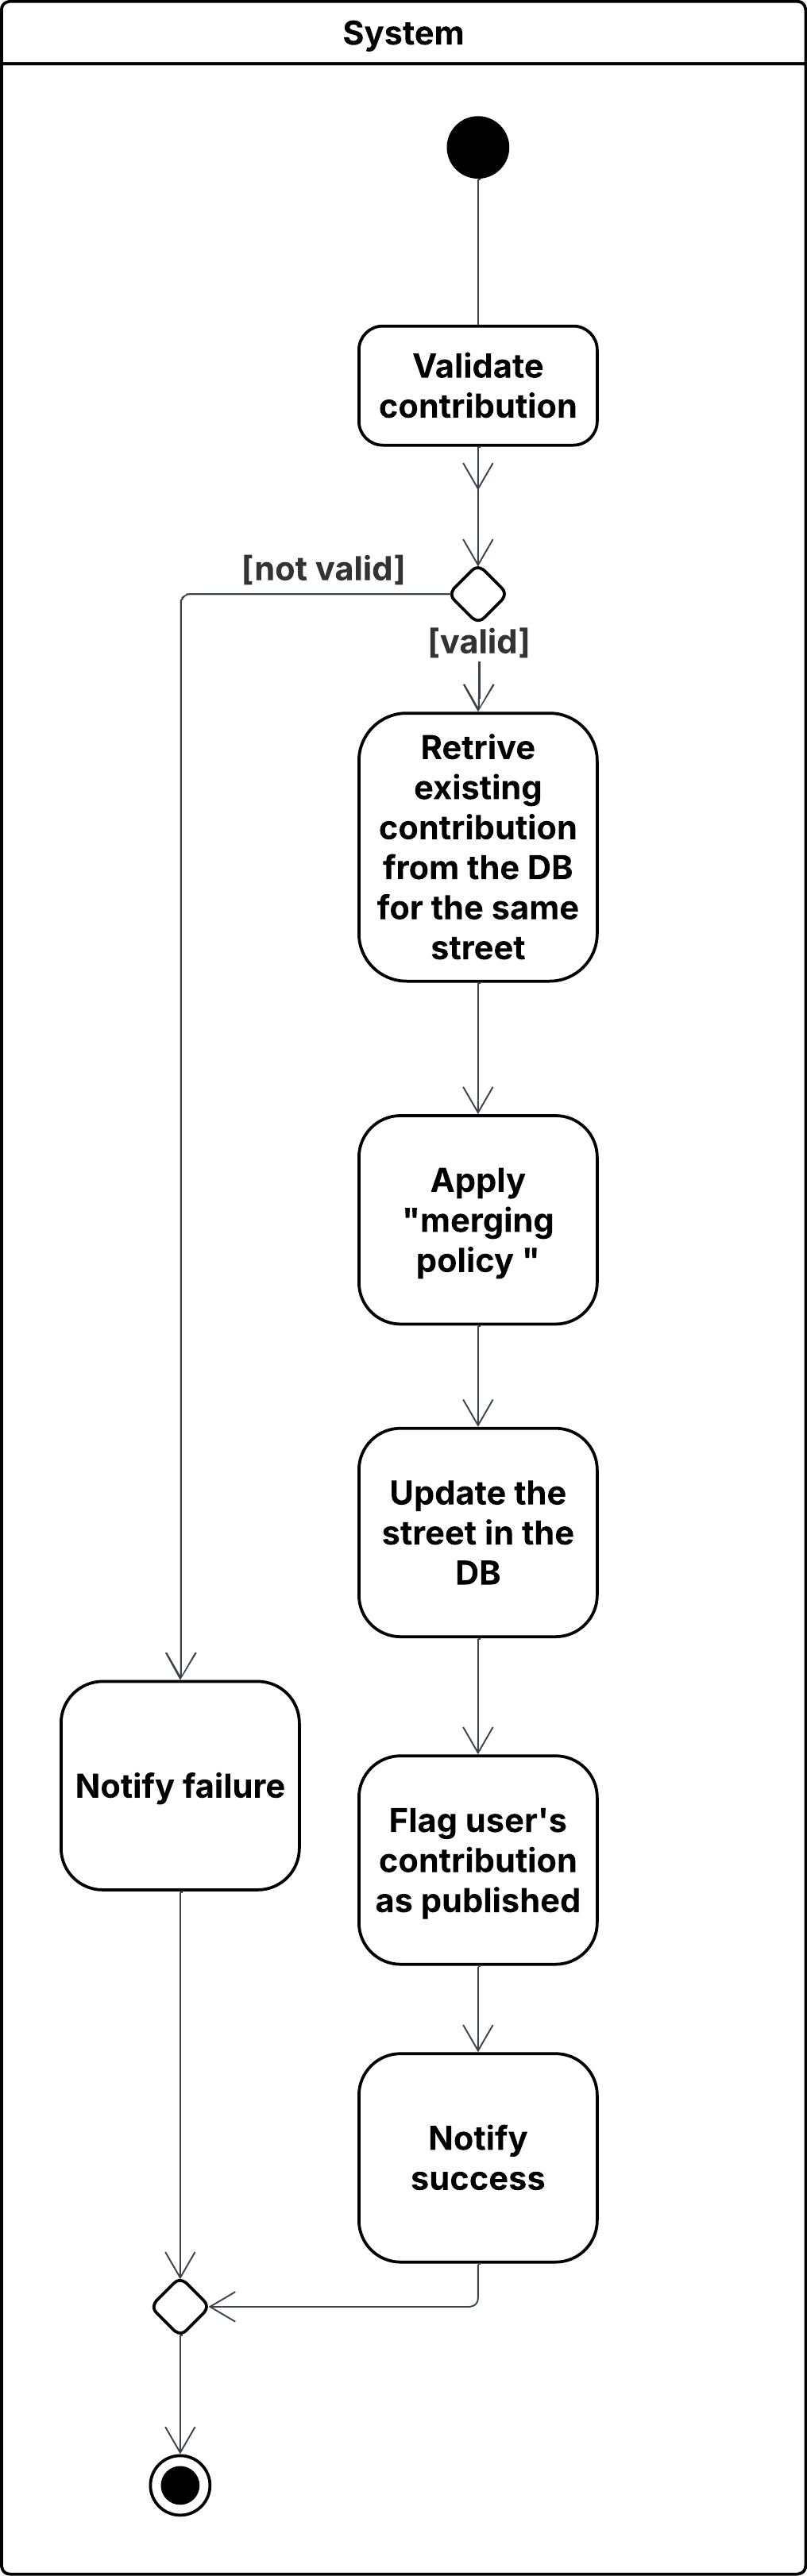
\includegraphics[width=0.4\linewidth]{RASD/Version1.0/images/activity diagram/UC7.png}
         \caption{Publish Contribution}
         \label{fig:publish_contribution}
     \end{center}
\end{figure}

\newpage


\subsubsection*{UC\cuc . View Map}
\begin{center}
    \begin{longtable}{|l|p{0.75\linewidth}|}
        \hline
        \textbf{Actor}            & User \\
        \hline
        \textbf{Entry Conditions} & The User is logged into the platform and has access to the map functionality. \\
        \hline
        \textbf{Flow of Events}    
        & \cucsteps. The User clicks on the ``Map'' section. \\
        & \cucsteps. The system loads the default map region (e.g., around the User's current position or last viewed area). \\
        & \cucsteps. The system retrieves the visible bike-path data for the current map region. \\
        & \cucsteps. The system displays the map together with the visible paths and their associated contributions (e.g., obstacles, warnings, roadworks). \\
        & \cucsteps. The User chooses an action on the map view (e.g., search for a path, tap on a displayed path segment, move around the map, or start following a path). \\
        & \cucsteps. If the User searches for a specific path or destination, the system invokes the \hyperref[search_path]{\uline{UC.~Search Path}} use case and, after the search is completed, updates the map with the best suggested paths (e.g., top 5). \\
        & \cucsteps. If the User taps on a displayed path, the system shows the selected path with more detailed information, including aggregated contributions along that path. \\
        & \cucsteps. If the User decides to follow a selected path, the system redirects the User to the ``Automatic trip mode'' page and invokes the \hyperref[sec:uc_follow_path]{\uline{UC.~Follow Path}} use case. \\
        & \cucsteps. If the User simply moves around the map (pan/zoom), the system retrieves bike-path data for the newly visible region and refreshes the map with updated paths and contributions. \\
        & \cucsteps. For readability, the activity diagram omits that the User can exit the map or return to previous sections of the application at any time during the interaction. \\
        \hline
        \textbf{Exit Conditions}   & The User has visualized the desired map area, inspected the available paths and related contributions, and optionally started following a selected path.\\
        \hline
        \textbf{Exceptions}       & {%
            \begin{itemize}[leftmargin=*]
                \item No bike-path data is available for the current map region: the system still displays the map but shows an informative message indicating that no paths are present.
                \item A temporary error occurs while retrieving path data or contributions: the system notifies the User of the failure and suggests retrying the operation.
            \end{itemize}
        } \\
        \hline
    \end{longtable}
\end{center}



\begin{figure}[H]
    \begin{center}
         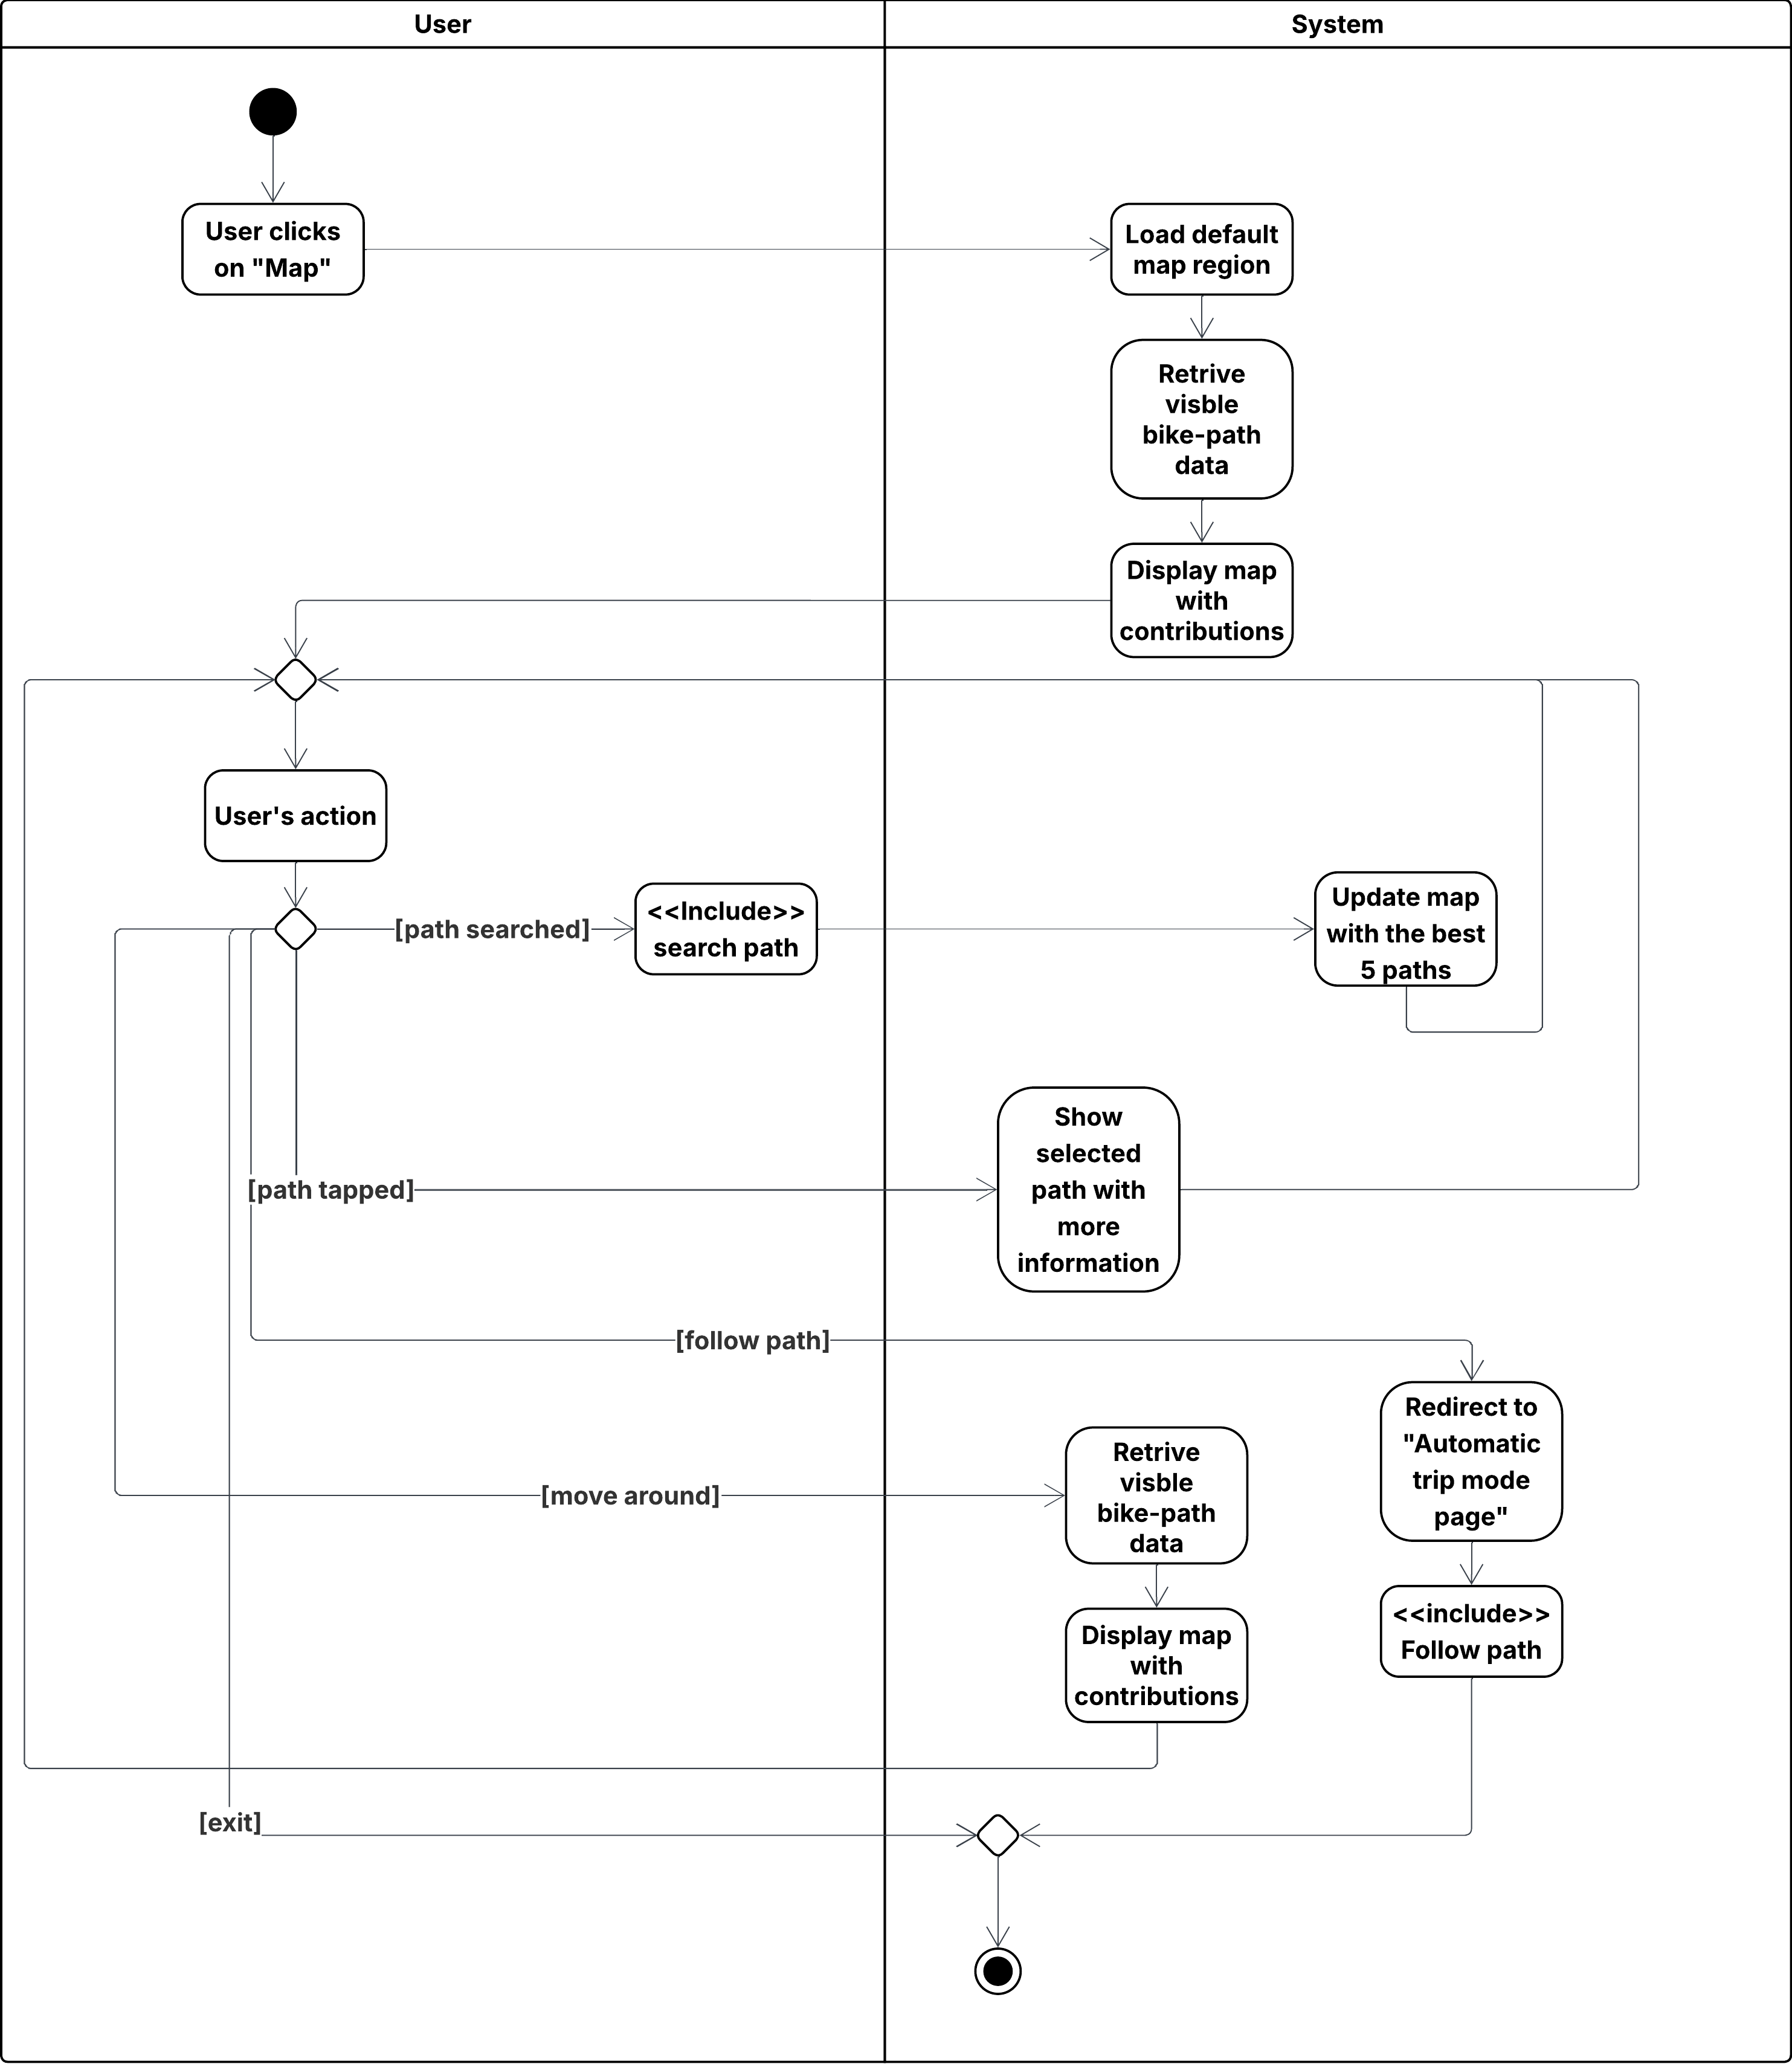
\includegraphics[width=1\linewidth]{RASD/Version1.0/images/activity diagram/UC8.png}
         \caption{View Map}
         \label{fig:view_map}
     \end{center}
\end{figure}

\newpage

\subsubsection*{UC\cuc . Search Path}
\label{sec:uc_search_path}
\begin{center}
    \begin{longtable}{|l|p{0.75\linewidth}|}
        \hline
        \textbf{Actor}            & User \\
        \hline
        \textbf{Entry Conditions} & The User is on a page where the map and the path search functionality are available (e.g., from \hyperref[view_map]{\uline{UC.~View Map}}). \\
        \hline
        \textbf{Flow of Events}    
        & \cucsteps. The User specifies the start and end points of the desired path (e.g., origin and destination on the map or via textual input). \\
        & \cucsteps. The system retrieves from the database the bike paths that connect the specified start and end points, if any exist. \\
        & \cucsteps. The system checks whether the User is registered or unregistered. \\
        & \cucsteps. If the User is registered, the system orders the retrieved paths according to the User's saved preferences and the trips recently completed by the User (e.g., preferred difficulty, usual routes). \\
        & \cucsteps. The system returns the list of searched bike paths to the invoking use case, already ordered if the User is registered. \\
        \hline
        \textbf{Exit Conditions}   & A set of bike paths matching the specified start and end points is produced and made available to the calling functionality.\\
        \hline
        \textbf{Exceptions}       & {%
            \begin{itemize}[leftmargin=*]
                \item No bike path exists connecting the specified start and end points: the system returns an empty result and may provide an informative message to the User.
                \item A temporary error occurs while retrieving paths from the database: the system notifies the failure and suggests the User to retry the search.
            \end{itemize}
        } \\
        \hline
    \end{longtable}
\end{center}




\begin{figure}[H]
    \begin{center}
         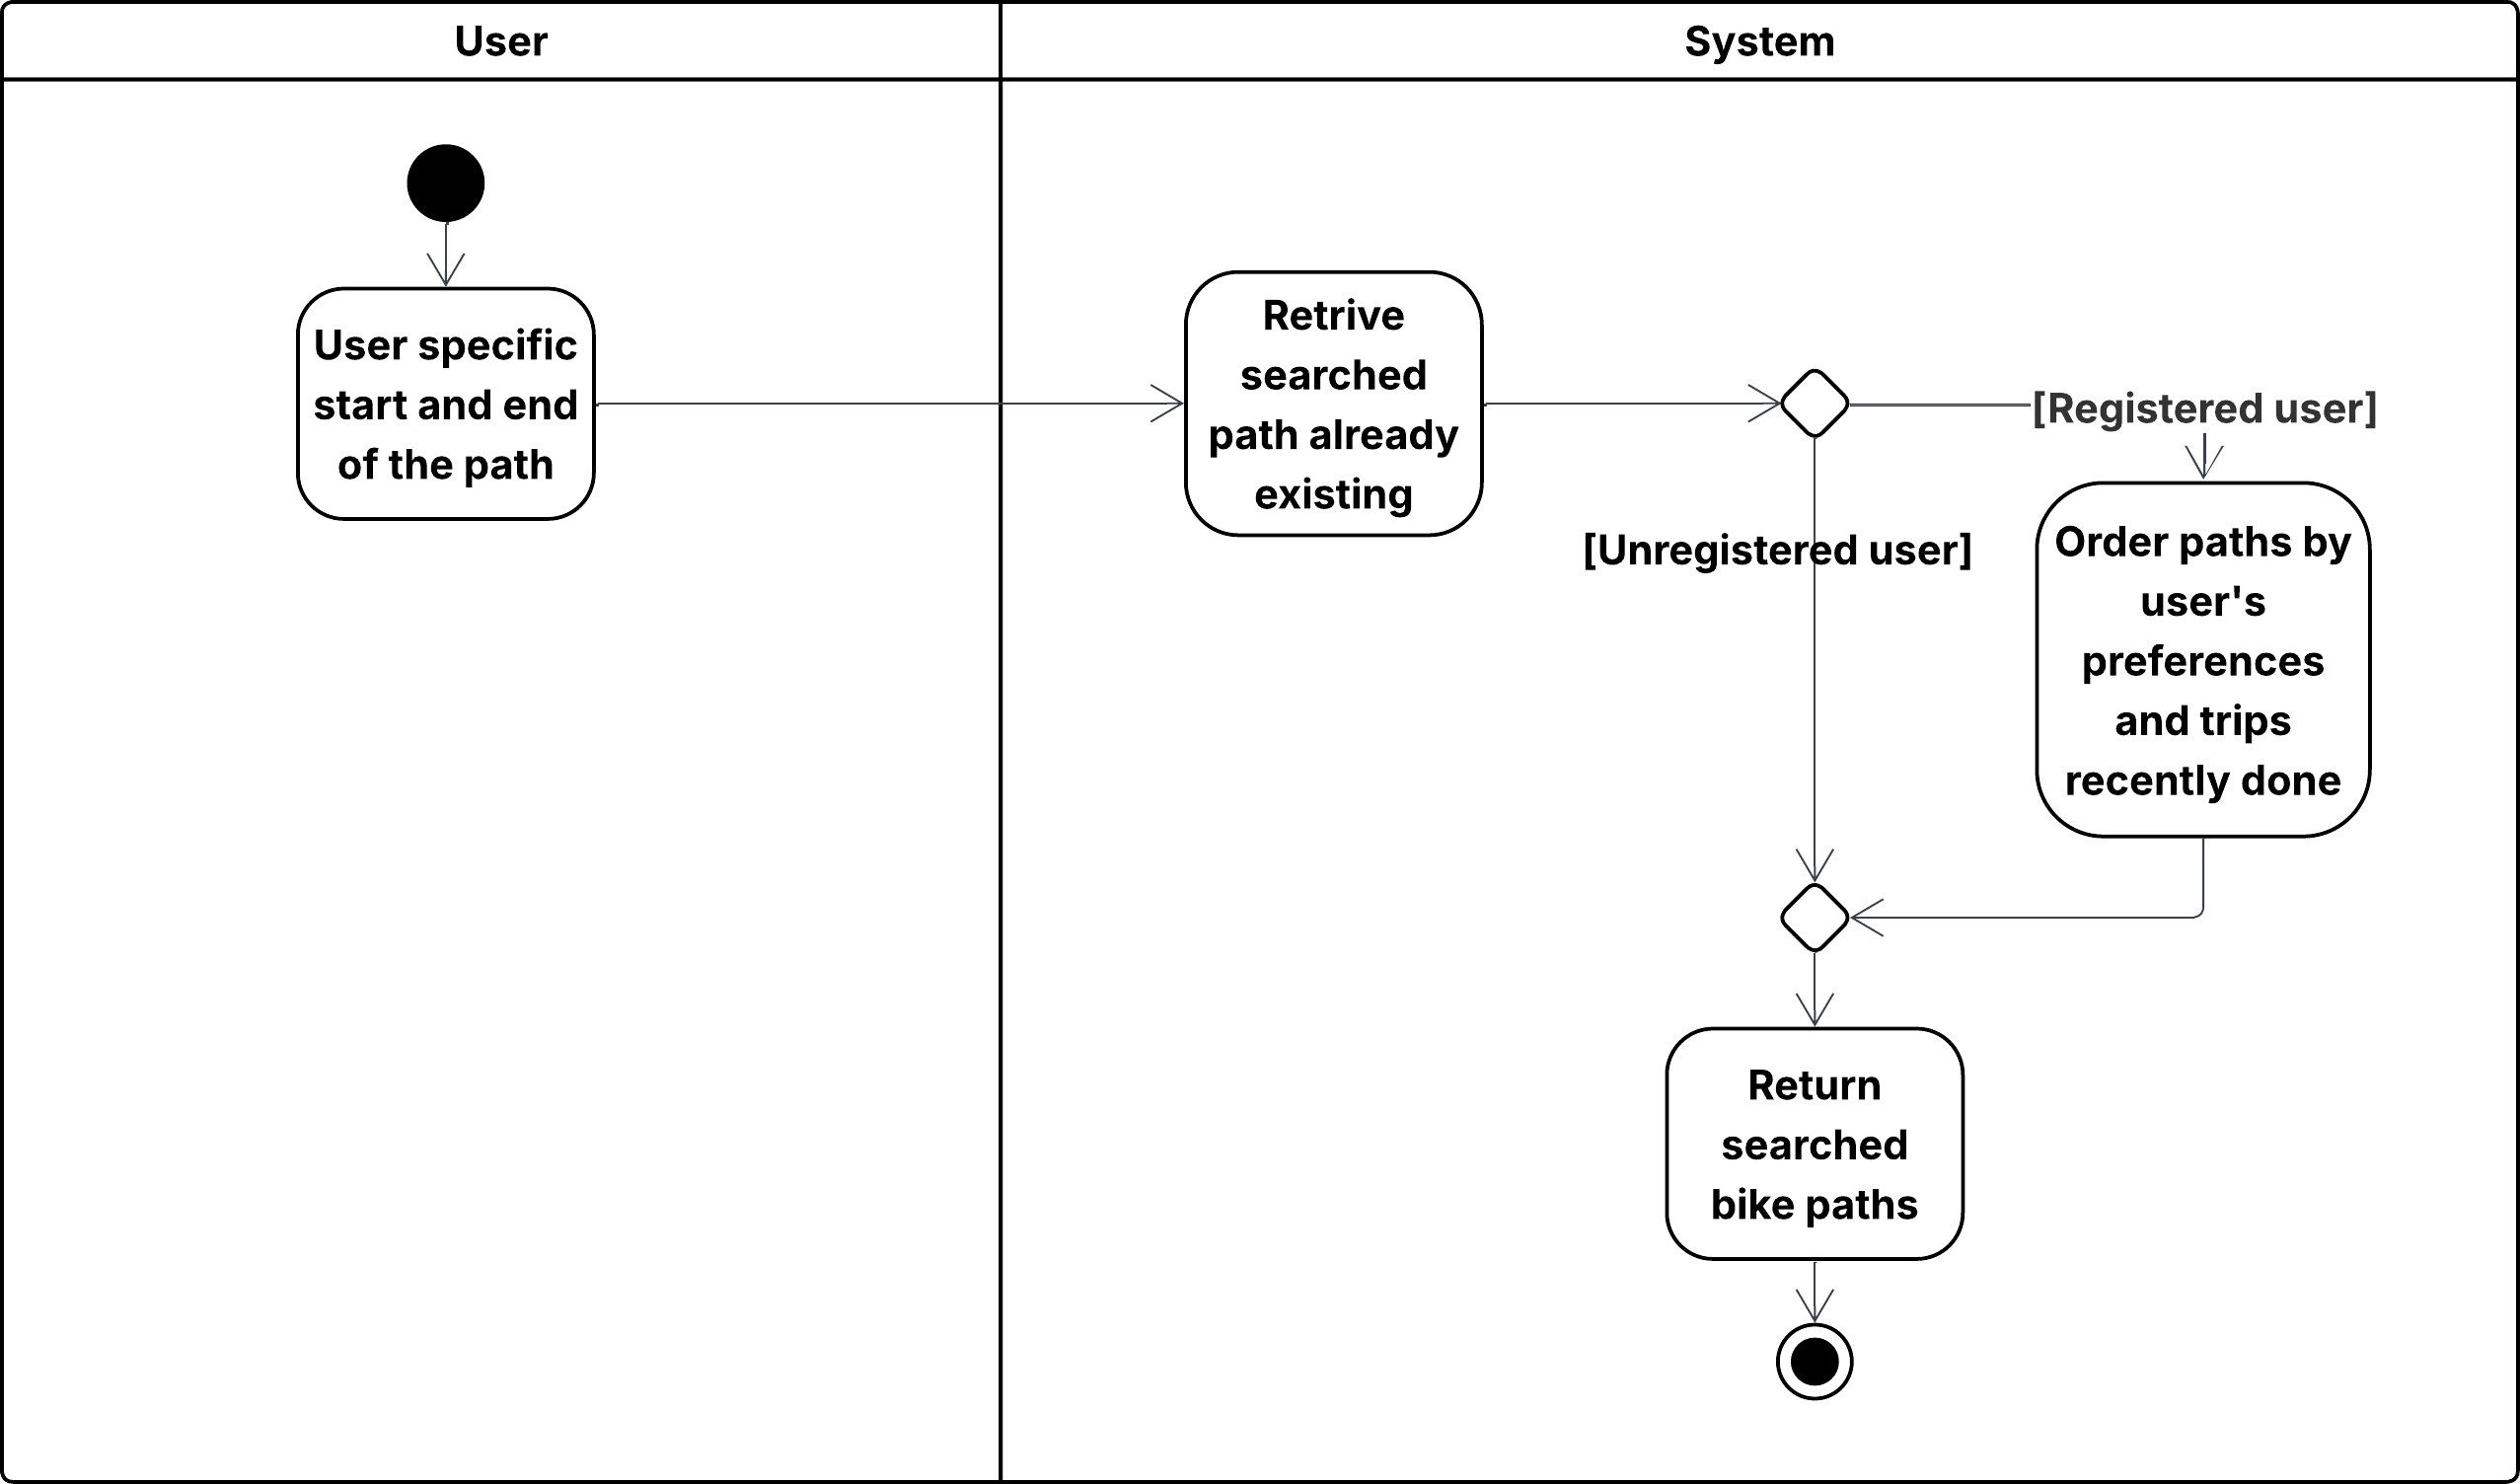
\includegraphics[width=0.8\linewidth]{RASD/Version1.0/images/activity diagram/UC9.png}
         \caption{Search Path}
         \label{fig:search_path}
     \end{center}
\end{figure}

\newpage



\subsubsection*{UC\cuc . Manual Insertion}
\begin{center}
    \begin{longtable}{|l|p{0.75\linewidth}|}
        \hline
        \textbf{Actor}            & Registered User \\
        \hline
        \textbf{Entry Conditions} & The Registered User is logged into the platform and has access to the manual trip insertion functionality. \\
        \hline
        \textbf{Flow of Events}    
        & \cucsteps. The system loads the default map region and initializes an empty \textit{TripDraft}. \\
        & \cucsteps. The User chooses how to add bike paths to the TripDraft (e.g., by manually selecting streets on the map or by searching for existing paths). \\
        & \cucsteps. If the User chooses to search for a path, the system invokes \hyperref[sec:uc_search_path]{\uline{UC.~Search Path}} and lets the User select one of the returned paths. \\
        & \cucsteps. For each selected or manually specified street, the system adds the corresponding bike path to the TripDraft and updates the map accordingly. \\
        & \cucsteps. The system asks the User whether the definition of the trip is finished; the User may repeat the previous step to add more streets. For readability, the activity diagram does not explicitly show that the User can also remove or adjust previously selected streets. \\
        & \cucsteps. Once the trip definition is complete, the system checks the validity of the TripDraft (e.g., at least one street, consistent geometry). If the TripDraft is not valid, the system shows an error and asks the User to correct it. \\
        & \cucsteps. The User chooses an action on the completed TripDraft (e.g., add contributions, save as trip, publish as report, or discard). \\
        & \cucsteps. If the User decides to add contributions, the User selects a street from the TripDraft and specifies a Contribution describing the status of that street (e.g., potholes, obstacles, roadworks). \\
        & \cucsteps. The system checks the validity of each added Contribution and, if a Contribution is not valid, removes it from the TripDraft and notifies the User. \\
        & \cucsteps. If the User chooses to save the TripDraft as a trip, the system saves the trip in the User's history and asks whether the associated Contributions should also be published (following the same iterative publication mechanism described for trips). \\
        & \cucsteps. If the User chooses to publish the information only as a report, the system treats the selected street and its Contribution as a standalone report, publishes the Contribution (without saving the TripDraft as a trip), and updates the corresponding path information. \\
        & \cucsteps. If the User chooses not to publish any Contribution, the system simply saves the trip in the User's history without publishing. \\
        & \cucsteps. If the User decides to discard the TripDraft, the system deletes all temporary data and terminates the use case. \\
        \hline
        \textbf{Exit Conditions}   & The User has either saved a manually defined trip (optionally with published Contributions), published one or more standalone reports about specific streets, or discarded the manual insertion.\\
        \hline
        \textbf{Exceptions}       & {%
            \begin{itemize}[leftmargin=*]
                \item The TripDraft is not valid (e.g., no street selected or inconsistent data): the system notifies the error and does not allow the User to save or publish until the trip is corrected.
                \item One or more Contributions added to the TripDraft are not valid (e.g., missing mandatory fields): the system removes the invalid Contributions and asks the User to review them.
                \item A temporary error occurs while saving the trip or publishing Contributions: the system notifies the failure and suggests the User to retry the operation.
            \end{itemize}
        } \\
        \hline
    \end{longtable}
\end{center}


\begin{figure}[H]
    \begin{center}
         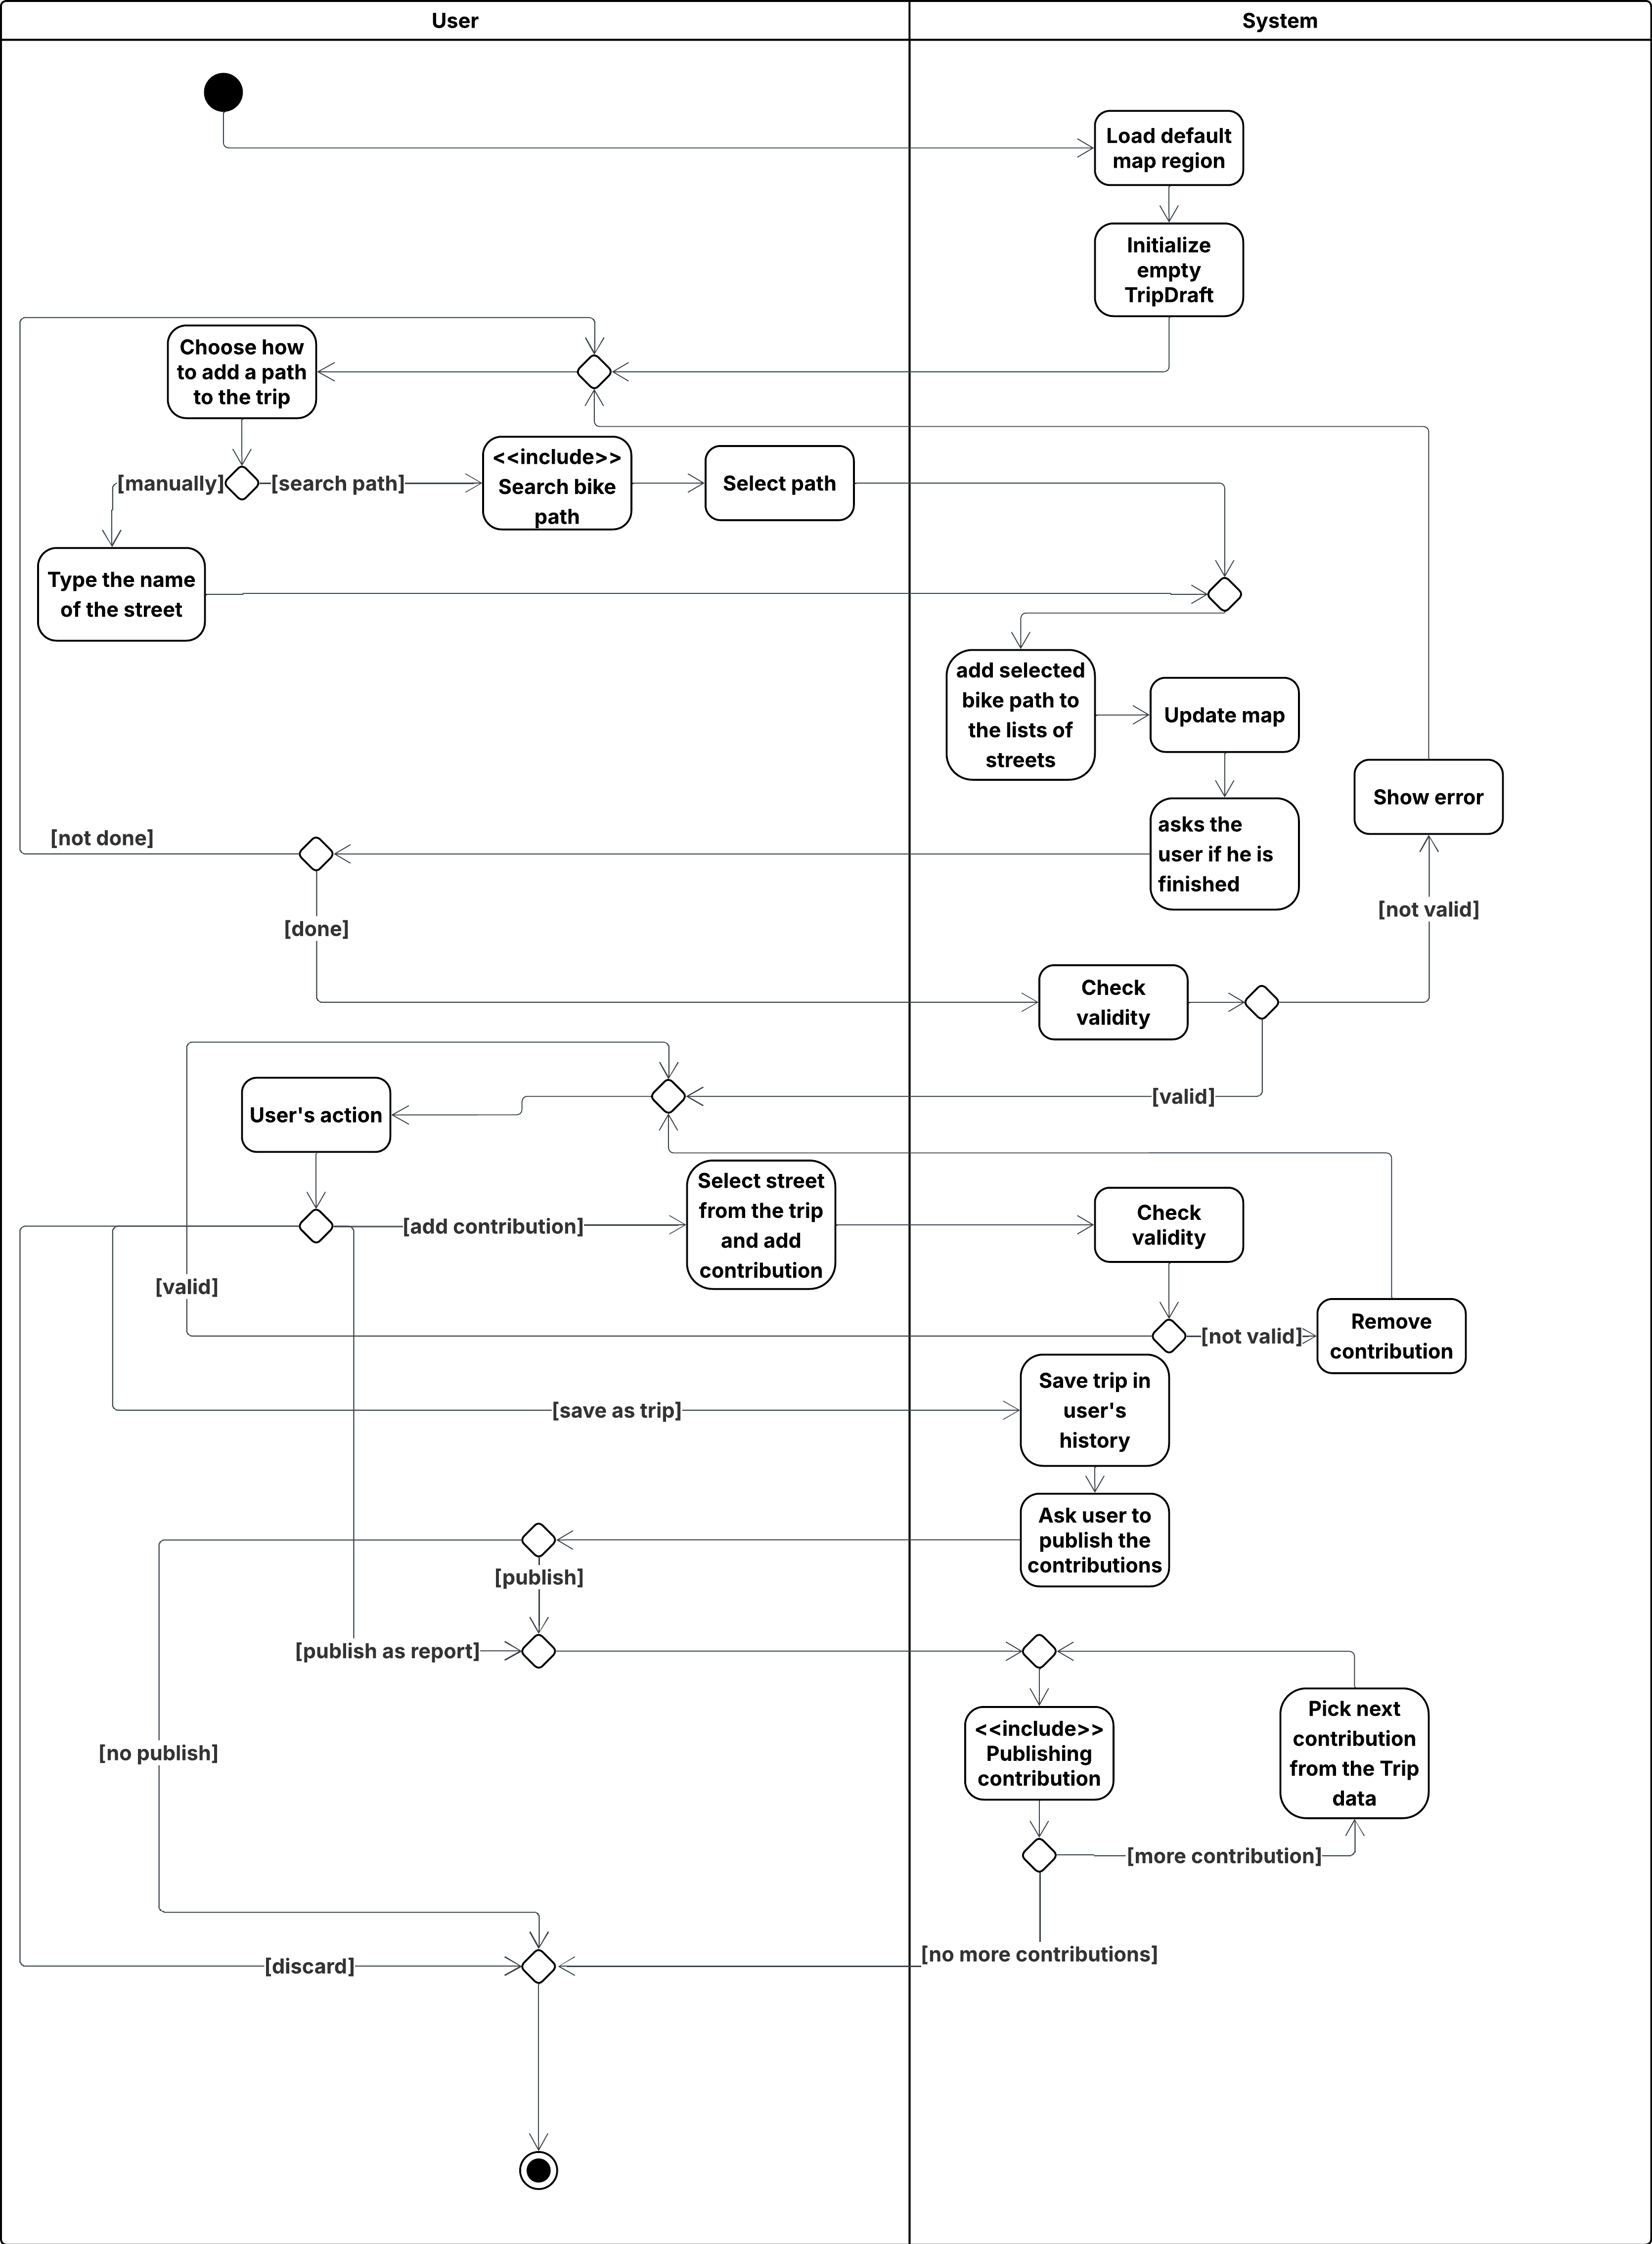
\includegraphics[width=1\linewidth]{RASD/Version1.0/images/activity diagram/UC10.png}
         \caption{Manual Insertion}
         \label{fig:manual_insertion}
     \end{center}
\end{figure}

\newpage

\subsubsection*{UC\cuc . Automatic Insertion}
\label{sec:uc_automatic_insertion}
\begin{center}
    \begin{longtable}{|l|p{0.75\linewidth}|}
        \hline
        \textbf{Actor}            
        & Registered User \\
        \hline
        \textbf{Entry Conditions} 
        & The Registered User is logged into the platform and has a device with GPS and motion sensors enabled. \\
        \hline
        \textbf{Flow of Events}    
        & \cucsteps. The User presses the ``Start recording'' button to begin an automatic trip. \\
        & \cucsteps. The system initializes a new \textit{RecordingSession} on the Client device. \\
        & \cucsteps. The system starts GPS tracking and activates accelerometer and gyroscope monitoring. \\
        & \cucsteps. While the recording is active, the system periodically acquires GPS samples and motion sensor data, storing them locally as raw trip data. \\
        & \cucsteps. In parallel, the system monitors the User’s movement to detect interruptions: consecutive GPS positions are compared and, if the distance travelled remains below a configurable threshold for a given time window, the User is marked as stationary; when movement resumes, the stationary status is cleared. \\
        & \cucsteps. The recording continues until the system receives an ``End recording'' event from the User. \\
        & \cucsteps. When the recording is stopped, the system stops GPS and motion sensors and finalizes the collection of raw trip data. \\
        & \cucsteps. The system reconstructs the full path of the trip from the collected GPS trace. \\
        & \cucsteps. Immediately after the recording phase, the system performs an inference process on the collected sensor data in order to generate a set of \textit{draft Contributions} associated with the reconstructed path. These Contributions are not published nor merged at this stage and are intended solely for User review. \\
        & \cucsteps. The system invokes the Data Enrichment Service, which computes aggregated trip statistics (e.g., distance, duration, speed profiles) and enriches the trip with external contextual information, such as weather data associated with the GPS trace, as described in \hyperref[sec:uc_enrich_trip_weather]{\uline{UC.~Enrich Trip with Weather Information}}. \\
        & \cucsteps. The system redirects the User to the ``Review and edit'' screen and includes \hyperref[sec:uc_edit_trip]{\uline{UC.~Edit Trip}}, allowing the User to inspect the automatically generated trip, modify its path if necessary, and edit, remove, or add Contributions before making any decision about saving or publishing the trip. \\
        \hline
        \textbf{Exit Conditions}   
        & An automatic trip has been recorded with its reconstructed path, a set of draft Contributions generated through post-processing inference, and enriched contextual and statistical information; control is transferred to the manual review and editing phase. \\
        \hline
        \textbf{Exceptions}       
        & {%
            \begin{itemize}[leftmargin=*]
                \item GPS or motion sensors are not available or cannot be started: the system notifies the User and does not start the automatic recording.
                \item A temporary error occurs while acquiring sensor data: the system attempts to continue recording with partial data and informs the User that some portions of the trip may be incomplete.
            \end{itemize}
        } \\
        \hline
    \end{longtable}
\end{center}






\begin{figure}[H]
    \begin{center}
         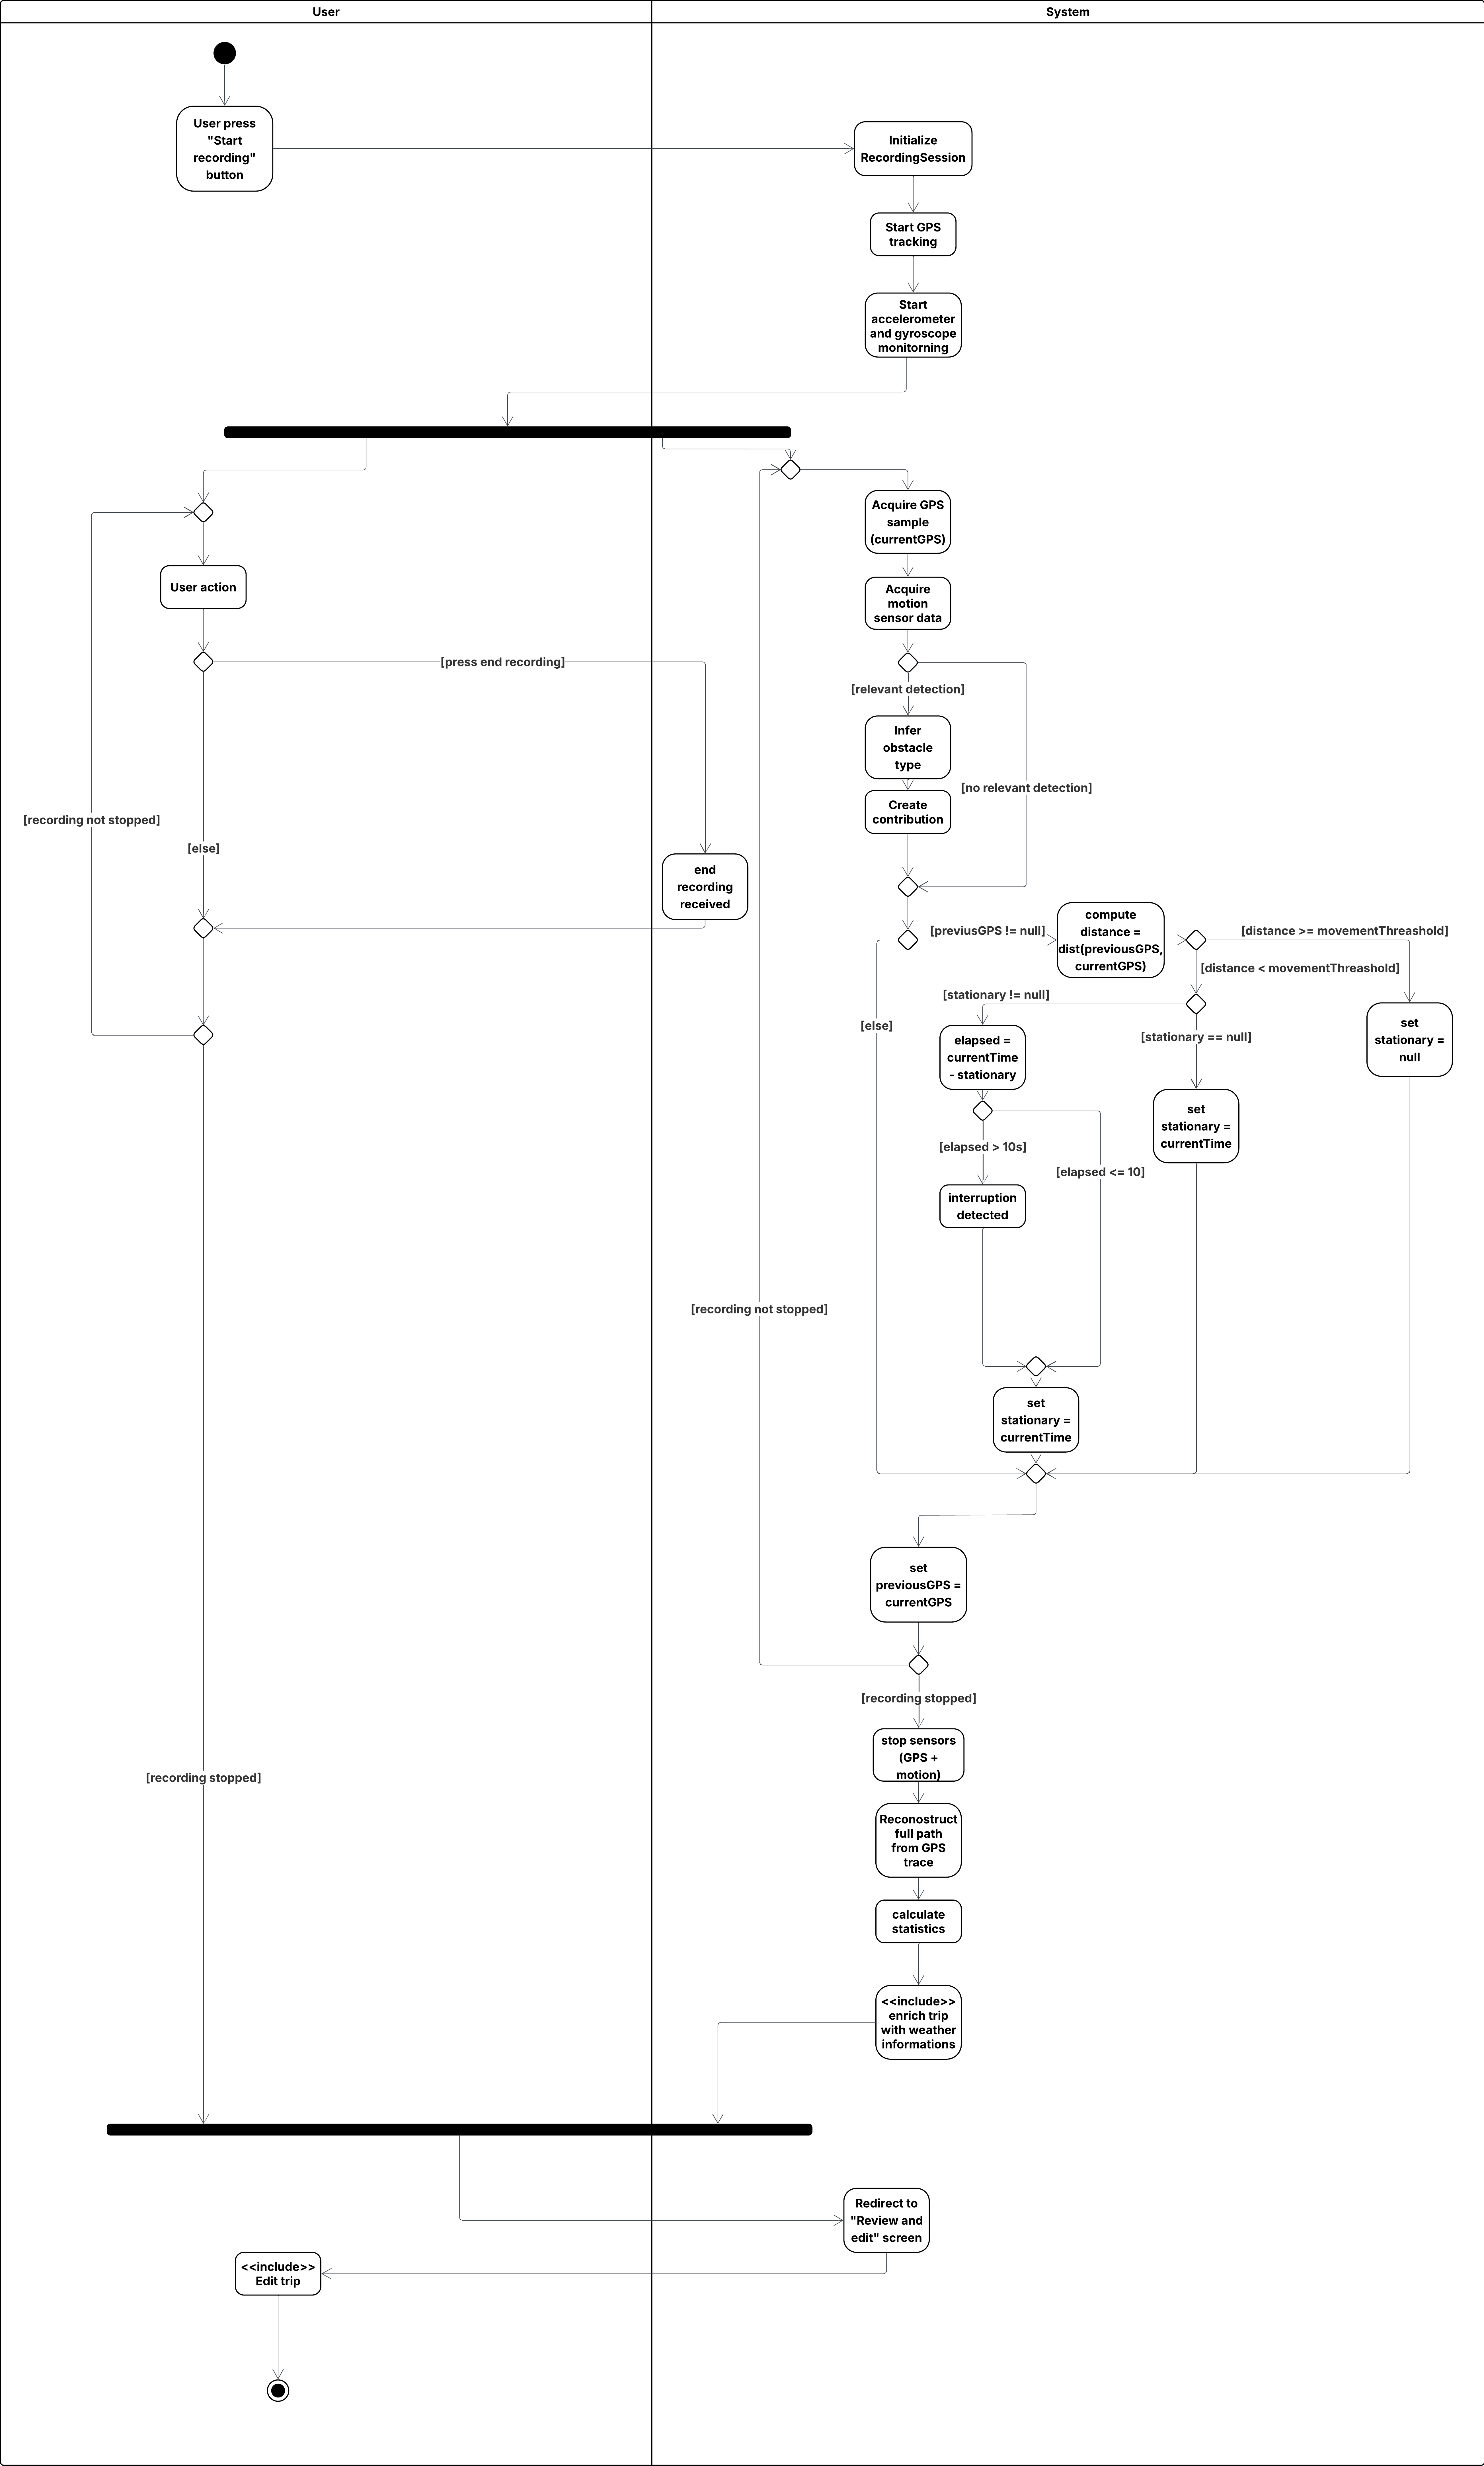
\includegraphics[width=0.85\linewidth]{RASD/Version1.0/images/activity diagram/UC11.png}
         \caption{Automatic Insertion}
         \label{fig:automatic_insertion}
     \end{center}
\end{figure}

\newpage

\subsubsection*{UC\cuc . Enrich Trip with Weather Information}
\label{sec:uc_enrich_trip_weather}
\begin{center}
    \begin{longtable}{|l|p{0.75\linewidth}|}
        \hline
        \textbf{Actor}            & System (Weather Service as external actor) \\
        \hline
        \textbf{Entry Conditions} & A TripDraft has been created and its GPS trace with timestamps is available. \\
        \hline
        \textbf{Flow of Events}    
        & \cucsteps. The system prepares a weather request using the trip's GPS trace and associated timestamps (e.g., start/end time and representative points along the route). \\
        & \cucsteps. The system sends the request to the external Weather Service API. \\
        & \cucsteps. The Weather Service receives the weather request. \\
        & \cucsteps. The Weather Service checks its availability for the given time and location. \\
        & \cucsteps. If the service is available, the Weather Service fetches the weather conditions corresponding to the requested time/place and returns the weather data to the system. \\
        & \cucsteps. If the service is not available or an internal error occurs, the Weather Service returns an error response to the system instead of weather data. \\
        & \cucsteps. Upon receiving the response, the system checks whether the request completed without errors. \\
        & \cucsteps. If no error occurred, the system attaches the retrieved weather data to the TripDraft so that it can be stored together with the trip and shown in the trip details. \\
        & \cucsteps. If an error occurred, the system marks the trip as ``no weather data available'' and continues without weather enrichment. \\
        \hline
        \textbf{Exit Conditions}   & The TripDraft is enriched with weather information associated with its GPS trace, or it is explicitly marked as having no weather data available.\\
        \hline
        \textbf{Exceptions}       & {%
            \begin{itemize}[leftmargin=*]
                \item The Weather Service is temporarily unavailable or returns an error: the system marks the trip as ``no weather data available'' and does not retry immediately.
                \item The GPS trace is incomplete or does not contain valid timestamps: the system does not send the request to the Weather Service and leaves the TripDraft without weather information.
            \end{itemize}
        } \\
        \hline
    \end{longtable}
\end{center}


\begin{figure}[H]
    \begin{center}
         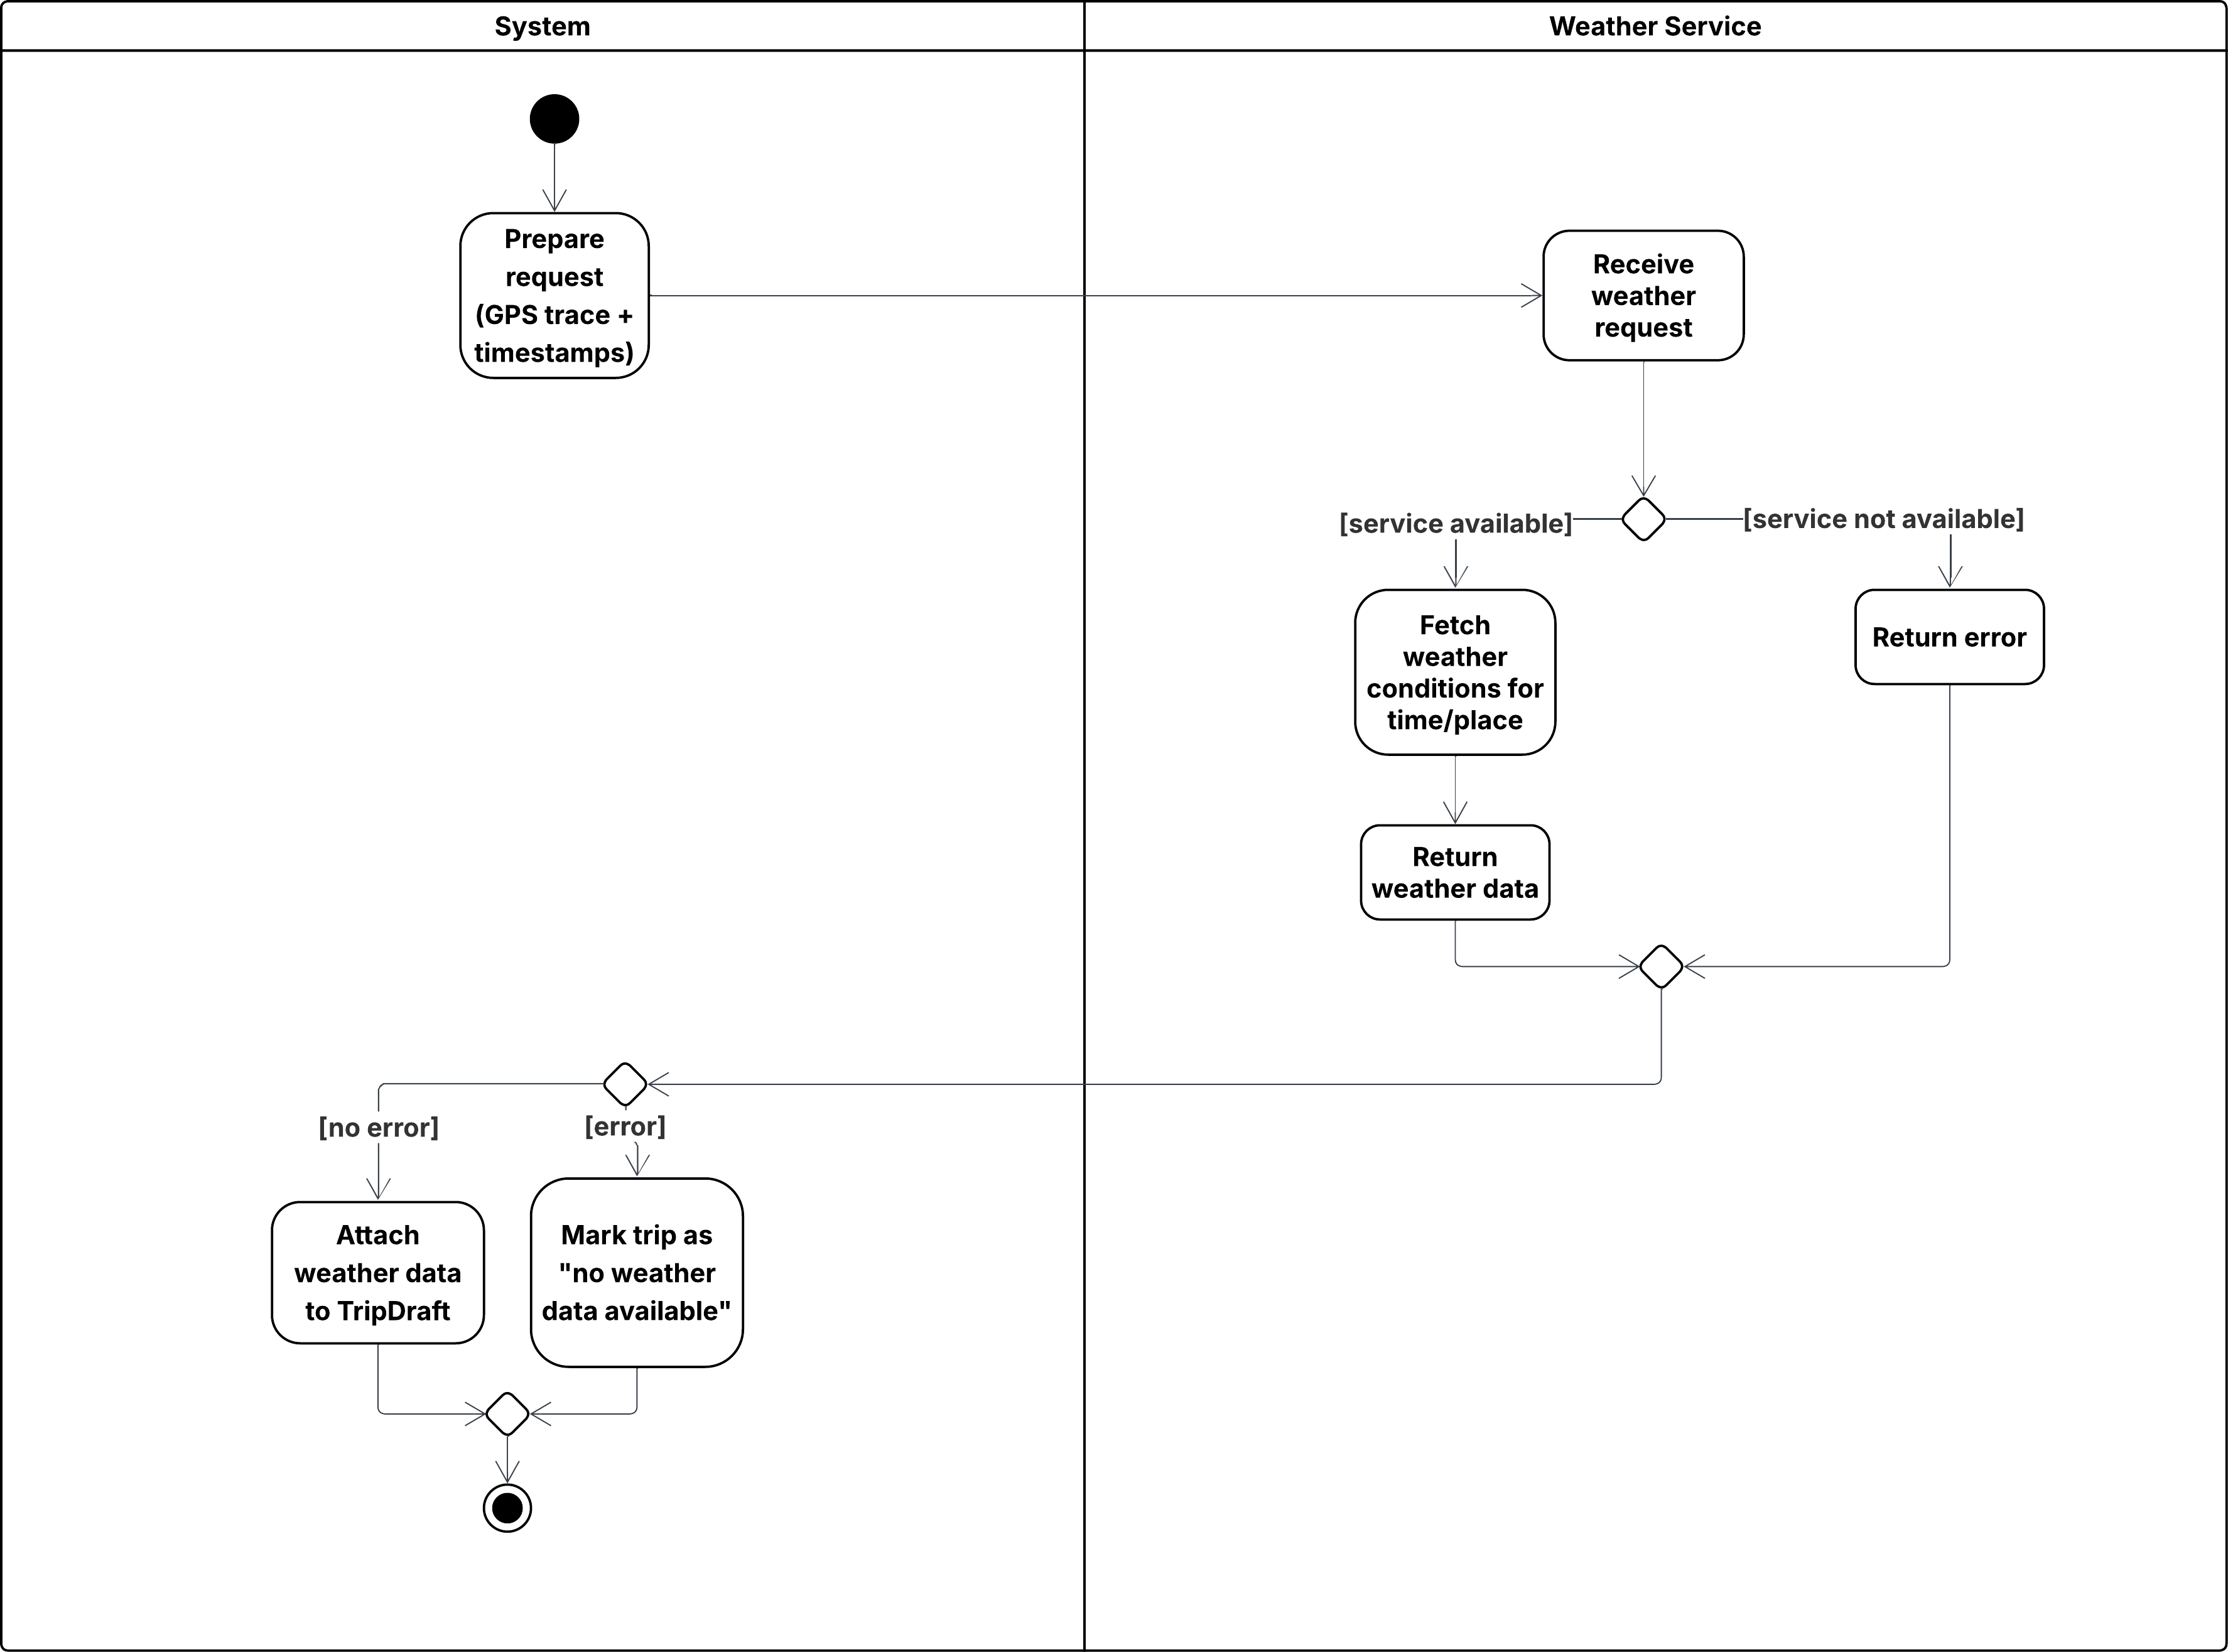
\includegraphics[width=1\linewidth]{RASD/Version1.0/images/activity diagram/UC12.png}
         \caption{Enrich Trip with Weather Information}
         \label{fig:uc_enrich_trip_with_weather_information}
     \end{center}
\end{figure}

\newpage



\subsubsection*{UC\cuc . Edit Trip}
\label{sec:uc_edit_trip}
\begin{center}
    \begin{longtable}{|l|p{0.75\linewidth}|}
        \hline
        \textbf{Actor}            & Registered User \\
        \hline
        \textbf{Entry Conditions} & A recorded trip (automatic defined) and its associated draft Contributions are available for review (at the end of recording). \\
        \hline
        \textbf{Flow of Events}    
        & \cucsteps. The system shows the trip together with the obstacles and Contributions that have been automatically detected. \\
        & \cucsteps. The User inspects the detected obstacles and Contributions and may confirm them, adjust their details, or remove the ones considered incorrect. \\
        & \cucsteps. The User can also add missing Contributions for streets included in the trip by selecting a street and specifying additional information (e.g., a new obstacle or warning). \\
        & \cucsteps. After reviewing the Contributions, the User chooses an action (e.g., store only, store and publish, or discard). \\
        & \cucsteps. If the User chooses to \textit{store and publish}, the system iteratively processes the Contributions associated with the trip: for each Contribution, the system invokes \hyperref[sec:uc_publish_contribution]{\uline{UC.~Publish Contribution}} and then selects the next Contribution until there are no more. \\
        & \cucsteps. Once all Contributions have been processed, the system stores the trip in the User's history together with the final set of Contributions. \\
        & \cucsteps. If the User chooses to \textit{store} without publishing, the system skips the publication step and only stores the trip and its Contributions in the User's history as private data. \\
        & \cucsteps. If the User decides to \textit{discard}, the system deletes the trip data and all associated draft Contributions, terminating the use case. \\
        \hline
        \textbf{Exit Conditions}   & The trip is either stored (with or without published Contributions) in the User's history, or it has been completely discarded.\\
        \hline
        \textbf{Exceptions}       & {%
            \begin{itemize}[leftmargin=*]
                \item An error occurs while storing the trip or its Contributions: the system notifies the User of the failure and suggests retrying the operation; no partial or inconsistent trip data is left saved.
                \item An error occurs during the publication of a Contribution (in the included UC Publish Contribution): the system notifies the User and leaves the affected Contribution in a non-published state while still allowing the rest of the trip to be stored.
            \end{itemize}
        } \\
        \hline
    \end{longtable}
\end{center}


\begin{figure}[H]
    \begin{center}
         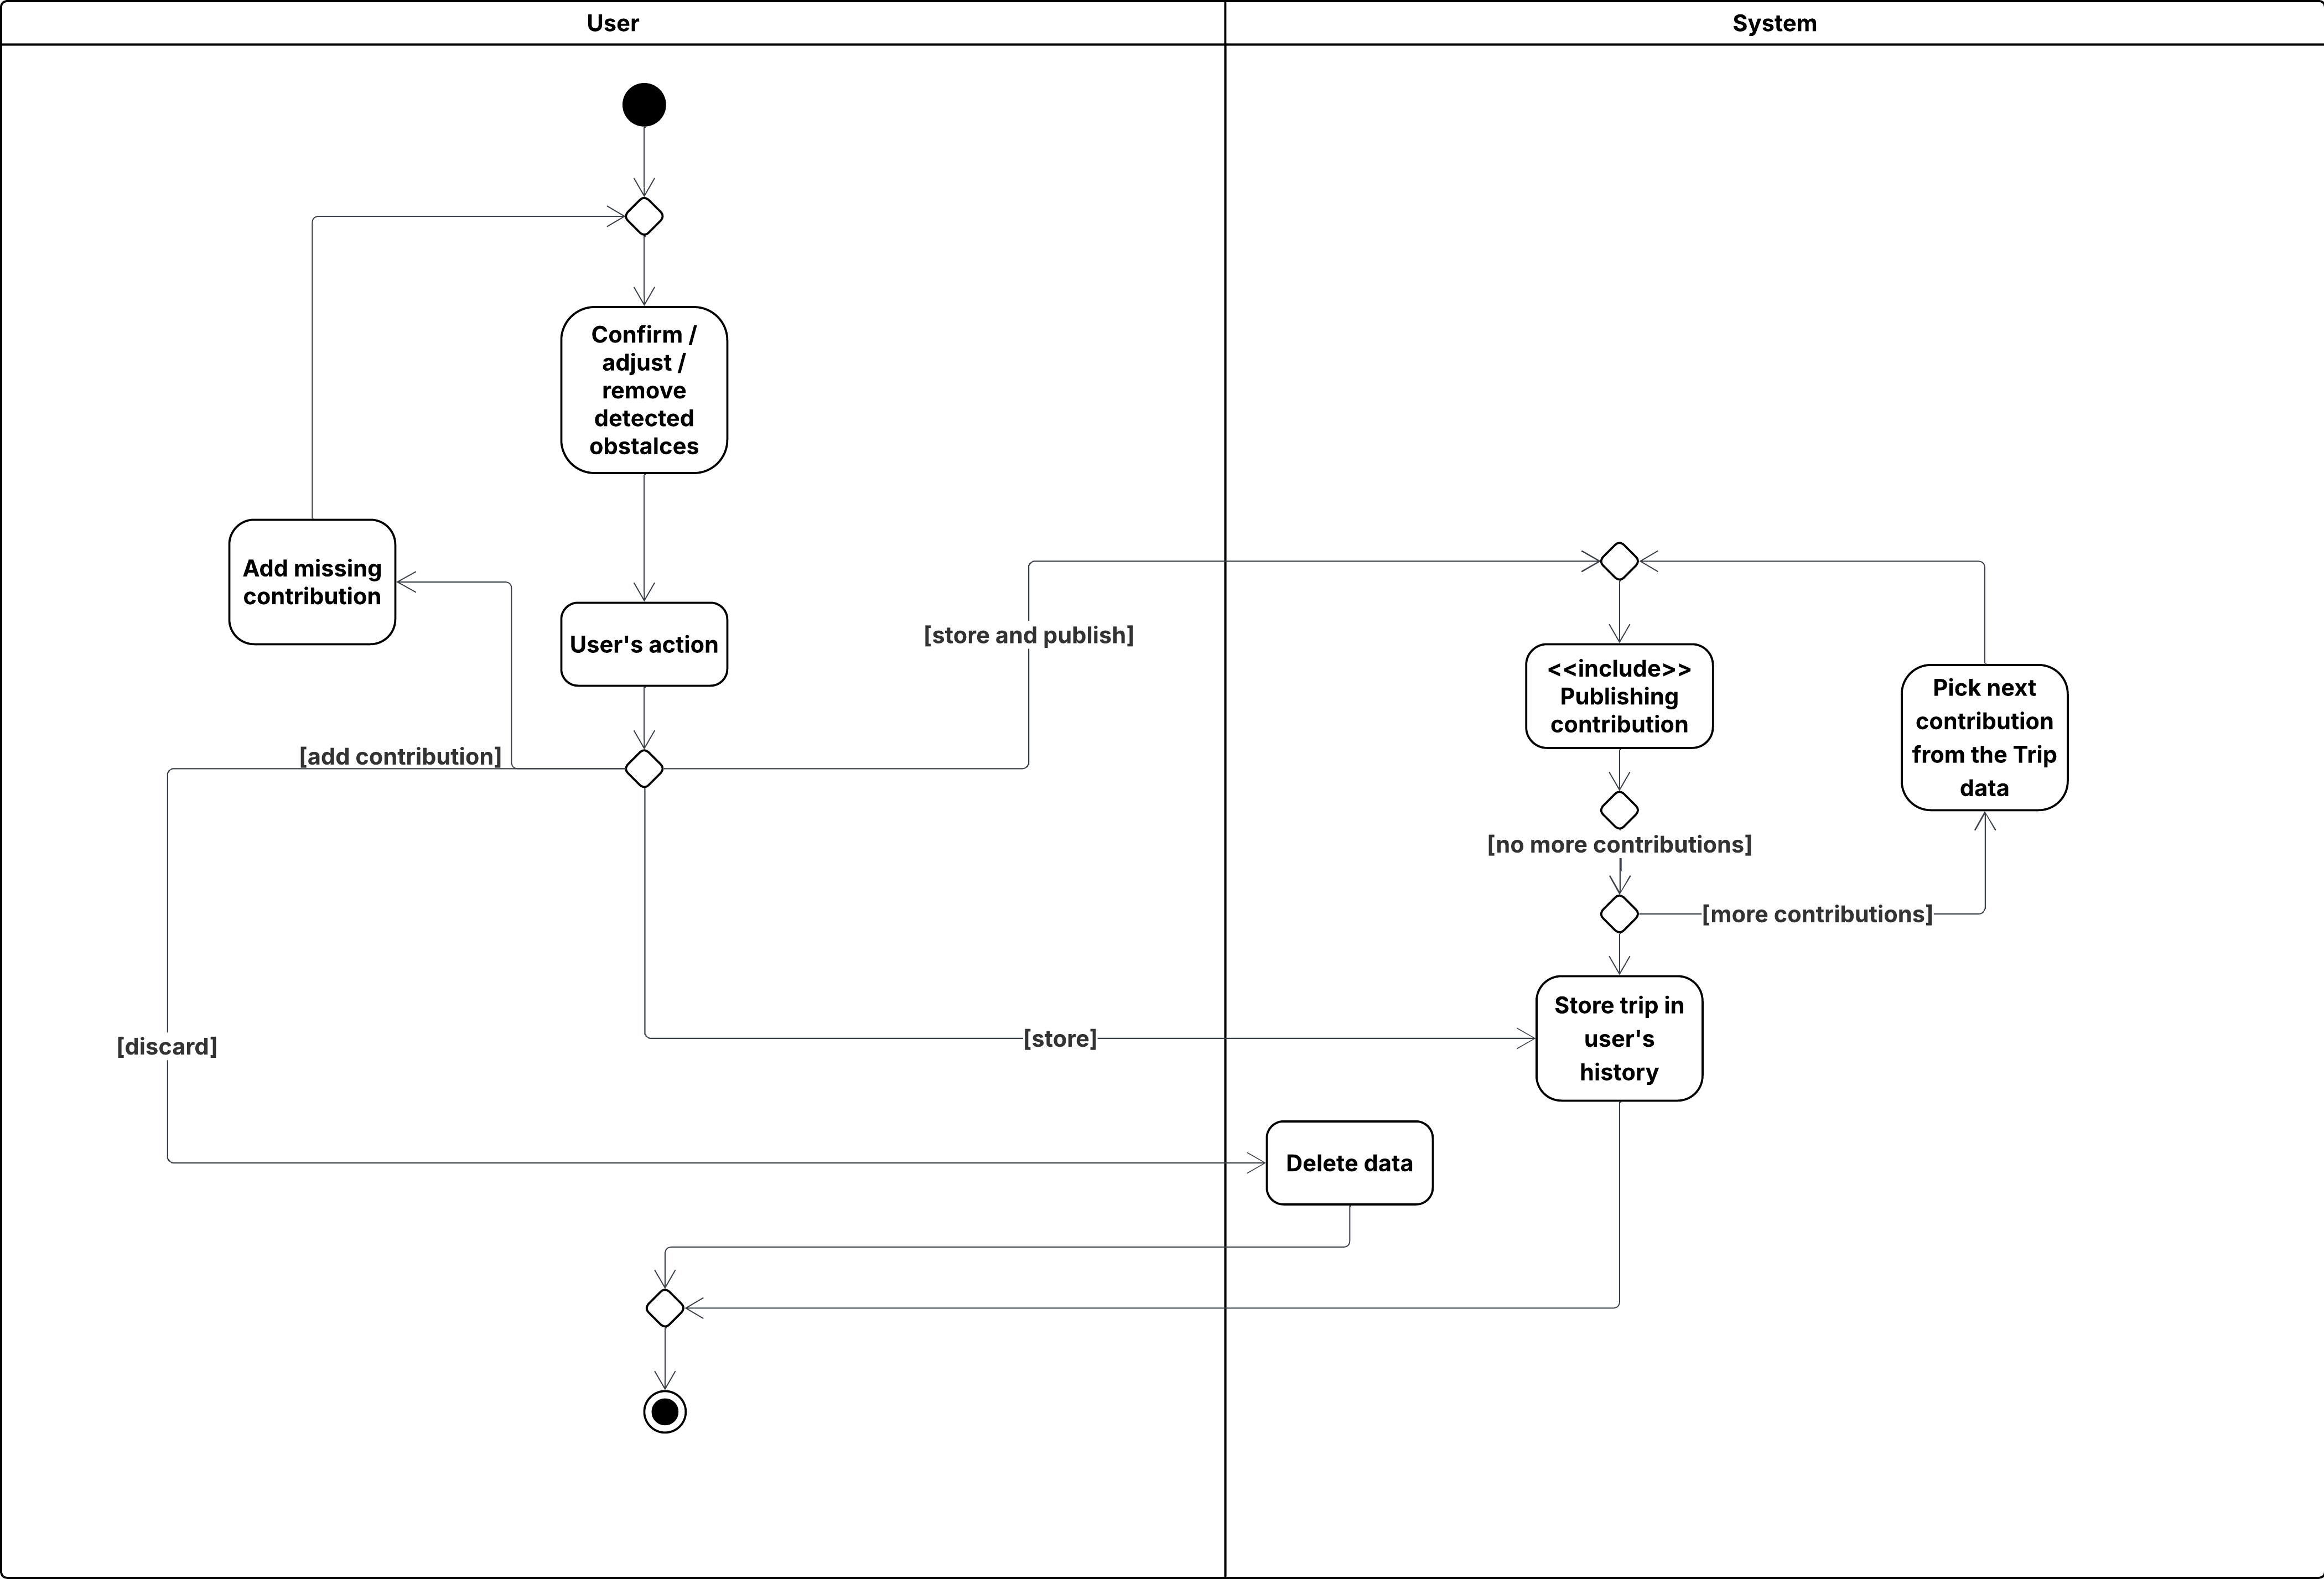
\includegraphics[width=0.9\linewidth]{RASD/Version1.0/images/activity diagram/UC13.png}
         \caption{Edit Trip}
         \label{fig:uc_edit_trip}
     \end{center}
\end{figure}

\newpage



\subsubsection*{UC\cuc . Follow Path (extends UC.~Automatic Insertion)}
\begin{center}
    \begin{longtable}{|l|p{0.75\linewidth}|}
        \hline
        \textbf{Actor}            & Registered User \\
        \hline
        \textbf{Entry Conditions} & 
        The User has selected a path from the map (see \hyperref[sec:uc_view_map]{\uline{UC.~View Map}}) and chooses to follow it. \\
        \hline
        \textbf{Flow of Events}    
        & \cucsteps. The system highlights the selected path on the map and opens a dedicated ``Follow path'' view. \\
        & \cucsteps. The User starts recording, triggering \hyperref[sec:uc_automatic_insertion]{\uline{UC.~Automatic Insertion}} for the current session. \\
        & \cucsteps. While the recording is active, the map keeps the chosen path visually highlighted; the User is free to follow it or deviate from it, and the system does not recompute or enforce the route. \\
        & \cucsteps. All other behaviours (trip recording, obstacle inference, interruption detection, reconstruction of the path, statistics computation and subsequent review/edit) follow exactly the flow described in UC.~Automatic Insertion. \\
        \hline
        \textbf{Exit Conditions}   & 
        An automatic trip has been recorded while a selected path was highlighted on the map; the resulting trip is then handled as in UC.~Automatic Insertion (review, edit, store, publish). \\
        \hline
        \textbf{Exceptions}       & {%
            \begin{itemize}[leftmargin=*]
                \item Sensors or GPS are not available: the system notifies the User and does not start the follow-path recording.
            \end{itemize}
        } \\
        \hline
    \end{longtable}
\end{center}
\noindent\textit{Remark.}
Since the behaviour of this use case is almost identical to \hyperref[sec:uc_automatic_insertion]{\uline{UC.~Automatic Insertion}},
apart from the highlighted path on the map and the absence of route recalculation, no dedicated activity diagram is provided.



\subsection{Mapping On Requirements}
\label{subsec:mapping_on_requirements}

\newcounter{row}
\setcounter{row}{1}
\newcommand{\crow} {\therow\stepcounter{row}}

\begin{longtable}{
    |>{\centering\arraybackslash}p{2cm}
    |>{\centering\arraybackslash}p{2.5cm}
    |>{\centering\arraybackslash}p{5cm}
    |>{\centering\arraybackslash}p{3.5cm}
    |>{\centering\arraybackslash}p{2.5cm}|
}
    \hline
    \textbf{Row ID} & \textbf{Goal ID} & \textbf{Req ID} & \textbf{DA ID} & \textbf{UC ID} \\ \hline
    \endfirsthead
    \hline
    \textbf{Row ID} & \textbf{Goal ID} & \textbf{Req ID} & \textbf{DA ID} & \textbf{UC ID} \\ \hline
    \endhead
    \hline
    \endfoot
    \hline
    \endlastfoot

    \crow & G1 & R1, R2, R3, R4 & DA3, DA4, DA5 & UC1, UC2, UC3, UC4, UC5 \\ \hline
    \crow & G2 & R2, from R5 to R13, R34, R35 & DA1, DA2, DA3, DA6, DA7, DA8, DA9, DA12, & from UC10 to UC14 \\ \hline
    \crow & G3 & R7, R8, R10, R14, R34, R35 & DA1, DA2, DA6, DA7, DA9, DA10, DA11 & UC6, UC13 \\ \hline
    \crow & G4 & R2, R10, R11, R12, R13 & DA3, DA12, DA13 & UC10, UC13 \\ \hline
    \crow & G5 & R2, R5, R6, R7, R8, R9, R10, R11, R34, R35 & DA3, DA6, DA7, DA9 DA10, DA11, & UC11, UC12, UC14 \\ \hline
    \crow & G6 & R2, from R15 to R20 & DA3 &  UC7 \\ \hline
    \crow & G7 & from R24 to R33 & DA1, DA2, DA3, DA11 & UC8, UC9 \\ \hline
    \crow & G8 & R19, R20, R21, R22, R23, R24 & DA1, DA2, DA14 & UC7\\ %\hline
    
    %\crow & G9 & R19, R21, R33, R34 & DA1, DA8, DA9, DA10, DA15, DA16 & UC7, UC10, UC11, UC14 \\ \hline
    %\crow & G10 & R20, R21, R23, R24--R30, R33, R34 & DA1, DA2, DA8, DA9, DA10, DA12, DA15, DA16 & UC7, UC8, UC9, UC10, UC11, UC14 

\label{tab:traceability}
\end{longtable}




\section{Performance Requirements}

The system gives real time information to its users, so it is critical that it provides a smooth and responsive user experience on mobile devices under normal operating conditions therefore:

\begin{itemize}
    \item The system shall provide a \textbf{responsive user interface}, ensuring that standard user interactions (e.g., navigation between screens, map panning and zooming, profile access) are completed within \textbf{0.5 seconds} under normal network conditions.
    
    \item Map rendering and updates, including the visualization of bike paths and aggregated contributions, shall be completed within \textbf{2 seconds} after the user changes the visible map area or performs a path search.
    
    \item The system shall support \textbf{real-time trip recording}, continuously collecting GPS and sensor data without causing noticeable delays, application freezes, or data loss during normal usage.
    
    \item Sensor data acquisition (e.g., GPS, accelerometer, gyroscope) shall not exceed acceptable latency thresholds that could compromise the accuracy of recorded trips or obstacle detection.
    
    \item The system shall be capable of handling \textbf{concurrent access by 15000 users} without degradation of core functionalities, such as map visualization, path search, and trip recording.
    
    \item Data synchronization between the mobile application and the backend server shall occur within a reasonable time frame, ensuring that newly recorded trips and contributions are available to the user within \textbf{30 seconds} after successful upload.
    
    \item The system shall ensure acceptable performance under varying network conditions, gracefully handling temporary connectivity issues by caching essential data locally and synchronizing it once the connection is restored.
\end{itemize}

\section{Design Constraints}

\subsubsection{3.4.1 Standards Compliance}
\begin{itemize}
    \item The system shall be developed in accordance with the guidelines and best practices for native mobile applications provided by \textbf{Android} and \textbf{iOS} platforms, including the official Android Developer Guidelines and Apple Human Interface Guidelines.
    
    \item The system shall comply with the \textbf{ISO/IEC/IEEE 29148:2018} standard for requirements engineering, ensuring consistency and traceability between requirements and design decisions.
    
    \item All data exchanged between the mobile application and backend services shall use secure communication protocols compliant with \textbf{HTTPS} and \textbf{TLS} standards.
    
    \item The system shall follow recognized \textbf{mobile security best practices}, including secure credential handling, encrypted local storage where required, and protection against common vulnerabilities such as unauthorized data access.
    
    \item The system shall adhere to applicable \textbf{data protection and privacy regulations}, including the \textbf{GDPR}, ensuring transparency in the collection, storage, and processing of personal and location-based data.
    
    \item The system shall comply with standard accessibility guidelines for mobile applications, such as the \textbf{WCAG 2.1} principles where applicable, to ensure usability for users with different abilities.
\end{itemize}

\subsubsection{3.4.2 Hardware Limitations}
\begin{itemize}
    \item The system shall operate within the hardware constraints typical of mobile devices, including limited CPU resources, memory, storage capacity, and battery life.
    
    \item The application shall be optimized to function correctly on devices with heterogeneous hardware configurations, ensuring acceptable performance on both high-end and mid-range smartphones.
    
    \item Continuous use of hardware components such as \textbf{GPS}, \textbf{accelerometer}, and \textbf{gyroscope} shall be managed efficiently to minimize battery consumption and prevent excessive resource usage.
    
    \item The system shall handle cases in which required hardware components are unavailable, disabled or denied by the user by providing appropriate feedback and gracefully degrading affected functionalities.
\end{itemize}


\section{Software System Attributes}

\subsubsection{3.5.1 Reliability}
\begin{itemize}
    \item The system shall ensure correct and consistent behavior during normal operation, minimizing unexpected crashes or data loss.
    
    \item The system shall preserve recorded trip data and user contributions in the presence of temporary failures, such as application restarts or network interruptions.
    
    \item The system shall detect and handle runtime errors, providing informative feedback to the user when an operation cannot be completed.
\end{itemize}

\subsubsection{3.5.2 Availability}
\begin{itemize}
    \item The system shall be available for use whenever the mobile device is operational and has network connectivity.
    
    \item Core functionalities such as trip recording and data visualization shall remain usable even during temporary backend unavailability, relying on local storage and deferred synchronization.
    
    \item The system shall support background execution, where permitted by the operating system, to ensure continuity of trip recording.
\end{itemize}

\subsubsection{3.5.3 Security}
\begin{itemize}
    \item The system shall protect user data by enforcing authentication mechanisms and secure session management.
    
    \item Sensitive information, including credentials and personal data, shall be transmitted exclusively through encrypted channels using HTTPS and TLS.
    
    \item The system shall restrict access to user-specific data, ensuring that each user can only view and modify their own information.
    
    \item The system shall request explicit user consent before accessing sensitive hardware components, such as GPS and motion sensors.
\end{itemize}

\subsubsection{3.5.4 Maintainability}
\begin{itemize}
    \item The system shall be designed following modular and layered architectural principles to facilitate maintenance and future enhancements.
    
    \item The codebase shall be documented and structured to support debugging, testing, and incremental updates.
    
    \item The system shall allow updates and bug fixes to be deployed without requiring changes to user data or system reconfiguration.
\end{itemize}

\subsubsection{3.5.5 Portability}
\begin{itemize}
    \item The system shall be portable across the supported mobile platforms, namely Android and iOS.
    
    \item Platform-specific components shall be isolated to minimize the effort required to adapt the application to different operating system versions.
    
    \item The system shall support future migration to additional mobile platforms with limited changes to the core application logic.
\end{itemize}



